%runningheads,
\documentclass[a4paper,USenglish,cleveref, autoref]{lipics-v2021}
%\usepackage{amsmath}
%\usepackage{amsfonts}

%\usepackage{tikz}
%\usetikzlibrary{shapes}
%\usepackage{cancel}
%\usepackage{latexsym}
%\usepackage{amsmath}
%\usepackage{comment}
%\usepackage{ amssymb }
%\usepackage{hyperref}
%\usepackage{float}
%\usepackage[left=3cm,right=3cm,top=3cm,bottom=3cm]{geometry}
%\usepackage[colorinlistoftodos]{todonotes}

\usepackage[color=green!40]{todonotes}
\usetikzlibrary{calc}
%\usetikzlibrary{patterns}
%\usepackage{ifthen}
 
\usepackage[utf8]{inputenc}

 \newcommand\DGP{\textsc{Dense Graph Partition}}
  \newcommand\MDGP{\textsc{Max Dense Graph Partition}}
 \newcommand\MUC{\textsc{Min Cut}}
 \newcommand\UC{\textsc{Min UnCut}}
 % \newcommand\RGC{\textsc{3-Regular-Cut\,}}



\newcommand{\defprob}[3]{
\begin{center}
%\fbox
{\begin{minipage}{.95\textwidth}
\noindent{\sc #1}\\\nopagebreak
{\bf Input:} #2 \\\nopagebreak
{\bf Question:} #3
\end{minipage}}
\end{center}
}

\newcommand{\commente}[1]{}


%Display of Figure (improve overleaf computing time)
\newcommand{\dispFig}[1]{#1}
%\newcommand{\dispFig}[1]{}

\newcommand{\convexpath}[2]{
	[   
	create hullnodes/.code={
		\global\edef\namelist{#1}
		\foreach [count=\counter] \nodename in \namelist {
			\global\edef\numberofnodes{\counter}
			\node at (\nodename) [draw=none,name=hullnode\counter] {};
		}
		\node at (hullnode\numberofnodes) [name=hullnode0,draw=none] {};
		\pgfmathtruncatemacro\lastnumber{\numberofnodes+1}
		\node at (hullnode1) [name=hullnode\lastnumber,draw=none] {};
	},
	create hullnodes
	]
	($(hullnode1)!#2!-90:(hullnode0)$)
	\foreach [
	evaluate=\currentnode as \previousnode using \currentnode-1,
	evaluate=\currentnode as \nextnode using \currentnode+1
	] \currentnode in {1,...,\numberofnodes} {
		-- ($(hullnode\currentnode)!#2!-90:(hullnode\previousnode)$)
		let \p1 = ($(hullnode\currentnode)!#2!-90:(hullnode\previousnode) - (hullnode\currentnode)$),
		\n1 = {atan2(\y1,\x1)},
		\p2 = ($(hullnode\currentnode)!#2!90:(hullnode\nextnode) - (hullnode\currentnode)$),
		\n2 = {atan2(\y2,\x2)},
		\n{delta} = {-Mod(\n1-\n2,360)}
		in 
		{arc [start angle=\n1, delta angle=\n{delta}, radius=#2]}
	}
	-- cycle
}



\bibliographystyle{plainurl}


\title{Dense Graph Partitioning on sparse and dense graphs}
\titlerunning{Dense Graph Partitioning}  

 
\author{Cristina Bazgan}{Universit\'e   Paris-Dauphine, PSL Research University, CNRS,UMR  7243, LAMSADE, 75016 Paris, France}{cristina.bazgan@dauphine.fr}{https://orcid.org/0000-0002-5460-6222}{}
 

 \author{Katrin Casel}{Hasso Plattner Institute, University of Potsdam,  Germany \and \url{https://hpi.de/friedrich/people/katrin-casel.html}}{Katrin.Casel@hpi.de}{https://orcid.org/0000-0001-6146-8684}{}
 
 
 \author{Pierre Cazals}{Universit\'e   Paris-Dauphine, PSL Research University, CNRS,UMR  7243, LAMSADE, 75016 Paris, France}{pierre.cazals@dauphine.eu}{https://orcid.org/0000-0002-7681-476X}{}
 
 
 \Copyright{Cristina Bazgan, Katrin Casel, and Pierre Cazals}
 
 
 \ccsdesc{Mathematics of computing~Combinatorial optimization}
 \ccsdesc{Mathematics of computing~Graph algorithms}
 \ccsdesc{Discrete Mathematics~Approximation algorithms}
  
 
 \authorrunning{C. Bazgan, K. Casel and P. Cazals}
 
% \author{
% Cristina Bazgan\inst{1} \orcidID{0000-0002-5460-6222} \and
% Katrin Casel\inst{2} \orcidID{0000-0001-6146-8684} \and 
% Pierre Cazals\inst{1} \orcidID{0000-0002-7681-476X}
%}

% \authorrunning{Bazgan, Casel \& Cazals}
% \institute{
% Universit\'e   Paris-Dauphine, PSL Research University, CNRS,
%  UMR  7243, LAMSADE, 75016 Paris, France\\
% \email{cristina.bazgan@dauphine.fr, pierre.cazals@dauphine.eu},
% \and 
% Hasso Plattner Institute, University of Potsdam, Potsdam, Germany\\
% \email{Katrin.Casel@hpi.de}
% }

\keywords{NP-hardness, approximation, density, graph partitioning, bipartite graphs, cubic graphs, dense graphs}

\begin{document}
 \nolinenumbers
\maketitle              

\begin{abstract}
We consider the problem of partitioning a graph into a non-fixed number of  non-overlapping subgraphs of maximum density. The density of a partition is the  sum of the densities of the subgraphs, where the density of the subgraph is  the ratio of its number of edges and its number of vertices. This problem, called Dense Graph Partition, is known to be NP-hard on general graphs and polynomial-time solvable on trees, and polynomial-time  2-approximable.

In this paper we study the restriction of Dense Graph Partition to particular sparse and dense graph classes. In particular, we prove that it is NP-hard on dense bipartite graphs as well as on cubic graphs. On dense bipartite graphs, we further show that it is W[2]-hard parameterized by the number of sets in the optimum solution. On dense graphs on $n$ vertices, it is polynomial-time solvable on graphs with minimum degree $n-3$ and NP-hard on $(n-4)$-regular graphs. We prove that it is  polynomial-time  $4/3$-approximable on cubic graphs and admits an efficient polynomial-time approximation scheme on $(n-4)$-regular graphs. 
\end{abstract}

%\todo{C: I don't know to put email adresses K: The at-symbol after the name is clickable and has the email}



\section{Introduction}


% With the advancement of social and other  types of networks and other complex systems, there has been a growing interest in the problem of finding communities in such structures.  


% *******************************


 
 
% \bigskip
% Darlay et al. remarked that if the number of partitions is fixed, minimizing the sparsity is equivalent to the $k$-means problem (if $\{u,v\} \in E$ then $w(uv) = 1$ else $w(uv) = 0$). In fact, \DGP~ is a subproblem and minimizing $k$-means has not been shown NP-complete in this case. We will show that it can be seen as a generalization of partition into $k$ clique. \todo{Where it is written this in the paper ? why DGP is a subproblem? }
% \todo[inline]{P : it was written by me long time ago, I talked about this sentence in darlay's paper "When the number of classes is fixed , the problem of minimizing (sparsity) is equivalent to the minimization of the famous $k$-means criterion (see for instance [5], [28]). In this case, the number of edges in a class is replaced by the sum of their weights in the definition of the density. This problem is shown to be NP-hard when the edges are weighted by the Euclidean distance"}
% \todo[inline]{As I recall, the papers he quotes don't show what he says in this but it was a long time ago and I'm not sure it's very important}

% \todo[inline]{\url{Max density subgbraph with constraint https://link.springer.com/article/10.1007/s10878-012-9465-z}, \url{https://link.springer.com/chapter/10.1007/978-3-319-15612-5_2}}
% \todo[inline]{Compare de nombre technique de partitionnement de graphe, semble etre une mine d'or : \url{http://www.numdam.org/item/RO_2008__42_4_469_0/}}

% % With the same density criterion, there is some work on finding the densest subgraph. This problem has be shown solvable in polynomial time by Goldberg \cite{bib:density:goldberg1984finding} but if the size of the subgraph is a part on the input, the problem becomes NP-hard even in bipartite or chordal graph \cite{bib:density:corneil1984clustering} (it can be seen as a generalization of $k$-clique).

% There is an other famous criterion of density, the edge density citation \cite{Diestel2005}. It consists in measuring the number of edges on the number of possible edges. Here, this is not relevant because a partition where each part is a single vertex would always be an optimal solution.

% \todo[inline]{Clustering methods based on density constraint have been introduced by Wishart in 1976 (\cite{intro:WishartDensityClustering}). The initial idea was to build classes around elements having many neighbors in a
% threshold graph associated to a distance on $S$. The considers many density measures, most of them more sophisticated than our. The article written by Gu\'enoche et al.,  give an overview of the job done in this field up to 2008.}
% *************************


The research around communities in social networks can be seen as a contribution to the well establish
research of clustering and graph partitioning. Graph partitioning problems have
been intensively studied with various measures in order to evaluate clustering quality, see e.g.~\cite{New2004,Sch2007,For2010,BulucMSS016}  for an overview. In the context of social networks, a ‘community’ is a collection of individuals who are relatively well connected compared to other parts of the social network graph and a ‘community structure’ corresponds to a partition of the whole social network into communities.

We consider a classical definition of the density of a subgraph induced by a subset~$S$ of vertices (see, for example,  \cite{bib:density:darlay2012DENSE,bib:density:goldberg1984finding}) given by the ratio between the number of edges and the number of vertices in $S$.  The density of a partition  is the sum of the densities of all its parts. 

For this definition of density, there are several papers on finding the densest subgraph. This problem was shown solvable in polynomial time by Goldberg~\cite{bib:density:goldberg1984finding} but if the size of the subgraph is a part on the input, the problem called \textsc{$k$-Densest Subgraph} becomes NP-hard even restricted to bipartite or chordal graphs~\cite{bib:density:corneil1984clustering}. The approximability of \textsc{$k$-Densest Subgraph} was also  studied, see~\cite{Khot06,FeigePK01,BhaskaraCCFV10}. 
% Goldberg [9] (also see [14]) proved that the densest subgraph problem can be solved optimally in polynomial time.  Research results was also done on densest subgraph problem  subject to size constraints.
 
 
% In the k-densest subgraph problem the objective is to find a densest
% subgraph induced over precisely k vertices. The problem  was shown to be NP-hard by [7], Khot [11] shows that that there does
% not exist any PTAS for the k-densest subgraph problem under a reasonable complexity
% assumption. In the direction of upper bounds, [7] provide an algorithm
% with an approximation factor of O(nθ) where θ < 1/3. More recently, [3] give an
% algorithm for the k-densest subgraph with an approximation factor of O(n1/4).
 
 
In this paper, we study the problem \MDGP{} of finding a partition $\mathcal{P} = \{ V_1, \dots, V_k\}$, $k \geq 1$, of a given undirected graph $G$, such that the density of the partition, denoted by $d(\mathcal{P})$, is maximised.
Note that the general concept of a community structure does not put any restriction on the
number of communities. We therefore address the problem \MDGP{} of finding a partition of maximum density, without fixing the number of classes of
the partition. 
%In this paper we address the problem \MDGP{} of finding a partition of maximum density, without fixing the number of classes of the partition. 
Indeed, when the number of classes is given, the problem is a generalization of a partition into $k$ cliques.  
%If you fix the partition to have k sets, then you get density (n-k)/2 if and only if the partition is into cliques.


%  \medskip
% \noindent
% \emph{Related works.}

Darley et al.~\cite{bib:density:darlay2012DENSE} studied   \MDGP, and its complement  {\sc Min Sparse Graph Partition}. They defined  the  sparsity of a partition $\mathcal{P}$ as $F(\mathcal{P})= \frac{|\mathcal{P}|}{2} + d(\mathcal{P})$ and the  problem {\sc Min Sparse Graph Partition} as finding a partition of a given undirected graph $G$ such that the sparsity of the partition is minimised. Observe that these two problems \MDGP{} and  {\sc Min Sparse Graph Partition} are duals in the sense that solving the first one on a graph $G$ is the same as solving the second one on the complement of $G$. In~\cite{bib:density:darlay2012DENSE} it is shown that both problems are NP-complete, and that there is no constant factor approximation for  {\sc Min Sparse Graph Partition} unless $P=NP$.  Moreover, a polynomial time algorithm for \MDGP{} on trees is given.
We point out that their proof of NP-completeness is a polynomial time reduction from \textsc{$k$-Coloring}. By construction, the same reduction when starting from \textsc{3-Coloring} on graphs of degree at most 4 (proved NP-complete in~\cite{GJS1976}) yields as instance of \MDGP{} a graph on $n$ vertices and of minimum degree greater than~$n-4n^{4/5}$. Thus it follows that  \MDGP{} is NP-complete restricted to graphs of minimum degree~$n-4n^{4/5}$.


Aziz et al.~\cite{bib:density:aziz2015welfare} studied the problem \textsc{Fractional Hedonic Game}, and more particularly the \textsc{Max Utilitarian Welfare} problem as the simple symmetric version of the game defined as follows. Let $N$ be a set of agents, the utility of $i \in N$ in a coalition $S \subseteq N$ is $u_i(S) = \tfrac 1{|S|}{\sum_{j \in S}u_i(j)}$ where $u_i(j)$ is such that $u_i(j) \in \{0,1\}$ for a simple game and $u_i(j) = u_j(i)$ for a symmetric one. For \textsc{Max Utilitarian Welfare} one tries to find a partition~$C$ of~$N$ into coalitions that maximizes $\sum_{S \in C}\sum_{i \in S}u_i(S)$. This game can be seen as a graph~$G$ where agents are  vertices and there is an edge between two agents $i$ and $j$ if and only if $u_i(j)=1$.
In this context, $u_i(S) = \tfrac 1{|S|}{\sum_{j \in S}u_i(j)} = \tfrac 1{|S|}deg_{G[S]}(u_i)$. We deduce that $\sum_{S \in C}\sum_{i \in S}u_i(S) =\tfrac 1{|S|} \sum_{S \in C}\sum_{i \in S} deg_{G[S]}(u_i) = \tfrac 1{|S|}\sum_{S \in C}  {2|E(S)|} = 2 \cdot d(C)$. Hence, the problems \textsc{Max Utilitarian Welfare} and \MDGP{} are equivalent to within a constant, which means that the 2-approximation for the former given in~\cite{bib:density:aziz2015welfare} directly translates to the latter.
%In~\cite{bib:density:aziz2015welfare} it is shown that \textsc{Max Utilitarian Welfare} admits a polynomial-time 2-approximation based on \textsc{Maximum Matching}. This result directly transfers to \MDGP.
 



\medskip
\noindent
\emph{Our contributions.}  The following overview summarises the results achieved in this paper concerning \MDGP{} (MDGP). 
\begin{itemize}
\item MDGP is trivially solvable on graphs of maximum degree 2, we prove its NP-hardness for 3-regular (cubic) graphs. 

\item We establish that on bipartite complete graphs an optimal partition  consists of one part, that is the whole graph. Moreover if the size of the two independent sets are relatively prime numbers then this optimal solution is unique. We use this result to show that MDGP is $W[2]$-hard with respect to (an upper bound on) the number of clusters in an optimal solution on dense bipartite graphs. Our reduction is polynomial and hence in particular implies the NP-hardness of MDGP on dense bipartite graphs.

\item MDGP is trivial on complete graphs since the optimal solution is the whole graph as one part of the partition. Moreover, as we previously explained, it is NP-hard on graphs of minimum degree $n-4n^{4/5}$.  We show that for graphs of minimum degree $\geq n-3$, the problem is solvable in polynomial time and any optimal solution has two parts.  Moreover on $(n-4)$-regular graphs, the problem becomes NP-hard. 

\item We show that MDGP admits an approximation with ratio $4/3$ on cubic graphs, and an eptas (i.e.~a $(1+\varepsilon)$-approxiation for any $\varepsilon >0$) on $(n-4)$-regular graphs, improving on the 2-approximation on general graphs~\cite{bib:density:aziz2015welfare}
%\MDGP is polynomial-time 2-approxiamble \cite{bib:density:aziz2015welfare}. We show that on cubic graphs and on $(n-4)$-regular graphs it is better approximable, that is $4/3$-approxiamble and $(1+\varepsilon)$-approxiamble for any $\varepsilon >0$.
\end{itemize}

Our paper is organized as follows. Notations and  formal definitions are given in
Section~\ref{sec2}. The study of (dense) bipartite graphs is established in Section~\ref{sec3}. Section~\ref{sec4} presents the results on cubic graphs. In Section~\ref{sec5} we study
dense graphs. %, that is graphs of minimum degree at least $n-4$. 
 Some conclusions are given at the end of the paper.



\section{Preliminaries}\label{sec2}
 In this paper we assume that all graphs are undirected, without loops or  multiple edges, and not necessary connected. We use $G=(V,E)$ to denote an undirected  graph with a set~$V$ of vertices and a set $E$ of edges.  We use $|V|$ to denote the number of vertices in $G$, i.e., the order of $G$, and we use $|E|$ to denote the number of edges in $G$, i.e., the size of $G$. We denote by $deg_G(v)$ the degree of $v\in V$ in $G$ that is the number of edges incident to $v$. 
The maximum degree of $G$, denoted by $\Delta(G)$, is the degree of the vertex with the greatest number of edges incident to it. The minimum degree of $G$, denoted by $\delta(G)$, is the degree of the vertex with the least number of edges incident to it. For any vertex $v\in V$, $N_G(v)$ is the set of neighbors of~$v$ in $G$ and $N_G[v]= N_G(v)\cup\{v\}$.  Moreover, $N_G(S)=\bigcup_{v \in S} N_G(v)$. For a  graph $G=(V,E)$  and a subset $S\subseteq V$ we denote by $E(S)$ the set of the edges of $G$ with both endpoints in~$S$. For a given  partition $\{A,B\}$  of $V$, we  denote  by $E(A,B) = \{uv \in E:~u \in A,~ v \in B\}$. Further, $G[S]$ denotes the graph induced by $S$, defined as $G[S]=(S, E(S))$.
   
 A triangle graph is  the cycle graph $C_{3}$ or  the complete graph  $K_{3}$. %\todo[inline]{A graph is called $C_4$-free if it contains no cycle of length four as an induced subgraph.}
 A diamond graph has 4 vertices and 5 edges, it consists of a complete graph $K_{4}$ minus one edge. A graph is called cubic  if all its vertices are of degree three. A  graph is bipartite if its vertices can be partitioned into two sets $A$ and $B$ such that every edge connects a vertex in $A$ to one in $B$. A complete bipartite graph  is a special kind of bipartite graph where every vertex of $A$ is connected to every vertex in $B$. A graph  on $n$ vertices is $\delta$-dense if its minimum degree is at least $\delta n$. A set of instances is called  dense if there is a constant $\delta >0$ such that all instances in this set are $\delta$-dense (this notion was introduced in \cite{AroraKK95} and called everywhere-dense).  

The density $d(G)$ of a graph $G=(V,E)$ is the ratio between the number of edges and the number of vertices in $G$, that is, $d(G)=\tfrac{|E|}{|V|}$. Moreover, for $S\subseteq V$, $d(S)=d(G[S])=\tfrac{|E(S)|}{|S|}$. We use $\mathcal{P}$ to denote a partition of the set $V$
 of vertices of $G$, that is,  $\mathcal{P} = \{ V_1, \dots, V_k\}$, where $\cup_{i=1}^k V_i = V$, and $V_i \cap V_j = \emptyset$ for each $i, j \in \{1, \dots, k\}$. Then the density of the partition $\mathcal{P}$ of $G$ is defined as  $d(\mathcal{P})=\sum_{i=1}^k d(G[V_i])$, where $G[V_i]$ is the subgraph of $G$ induced by the subset $V_i$ of vertices, that is, $G[V_i]= (V_i, E_i)$, $E_i = \{\{u,v\} : \{u,v\} \in E \land u,v\in V_i\}$.  
 
 
We study the problem of finding a partition $\mathcal{P} = \{ V_1, \dots, V_k\}$ of a given graph~$G$, such that $k \geq 1$  
and that, among all such partitions,  $d(\mathcal{P})$ is maximised. We refer to this problem as {\sc Max Dense Graph Partition} and we define its decision version as follows.

\begin{center}
\fbox{\begin{minipage}{.95\textwidth}
\noindent{\sc Dense Graph Partition}\\\nopagebreak
{\bf Input:} An undirected   graph $G=(V,E)$, a positive rational number $r$. \\\nopagebreak
{\bf Question:}  Is there a partition $\mathcal{P}$ such that $d(\mathcal{P}) \geq r$ ?
\end{minipage}}
\end{center}
 
We use some concepts from parameterized complexity and refer to~\cite{CFK+15,DowFel2013} for details of this terminology. A parameterized problem is a decision problem given together with a parameter, that is, an integer $k$ depending on the instance.
Such a parameterized problem is fixed-parameter tractable (fpt for short) if it can be solved in time $f(k)\cdot|I|^c$ for an instance $I$ of size $|I|$ with parameter $k$, where $f$ is a computable function and $c$ is a constant. If a parameterized problem is hard for the complexity class W[2], it is unlikely (under certain complexity theoretic assumptions) to be fixed-parameter tractable. An fpt-reduction between two parameterized problems~$P$ and $Q$ maps instances $(I,k)$ of $P$ to instances $(I',k')$ of $Q$ in time $f(k)|I|^{O(1)}$ for some computable functions $f$ and $g$, such that $k'\leq g(k)$ and $(I,k)$ is a yes-instance of~$P$ if and only if $(I',k')$
is a yes-instance of~$Q$. If problem $P$ is W[2]-hard, then such an fpt-reduction shows that $Q$ is W[2]-hard as well.

Given an optimization problem in NPO and an instance $I$ of this problem, we denote by $|I|$ the size of $I$, by $opt(I)$
the optimum value of $I$, and by $val(I, S)$ the value of a feasible solution $S$ of instance $I$. The performance ratio of $S$ (or
approximation factor) is $r(I, S) = \max  \{\frac{val(I,S)}{opt(I)},\frac{opt(I)}{val(I,S)}\}\geq 1$.  
For a function $f$, an algorithm is an $f(|I|)$-approximation, if for every instance $I$ of the problem, it returns a solution $S$
such that $r(I, S) \leq  f (|I|)$. Moreover if the algorithm runs in polynomial time in  $|I|$, then this algorithm gives a polynomial time $f(|I|)$-approximation.
We consider in this paper only polynomial time algorithms. When $f$ is a constant $\alpha$, the problem is polynomial-time $\alpha$-approximable. When $f=1+\varepsilon$, for any $\varepsilon >0$, the problem admits a polynomial-time approximation scheme. When the running time of an approximation scheme is of the form $O(g(1/\varepsilon)poly(|I|)$ the problem has an efficient polynomial-time approximation scheme (eptas). 

Before we start studying specific graph classes, we observe the following helpful structural properties that hold for {\sc Dense Graph Partition} on general graphs.
\begin{remark*}\label{remarkconnexe}
 We can assume that for any optimal partition  $\mathcal{P}$ and for any part $P_i \in \mathcal{P}$, $G[P_i]$ is connected, since otherwise turning each connected  component into its own part does not decrease the density.
\end{remark*}

 \begin{lemma}\label{lemmacomplete}
   Among all partitions of $G$ into $t\geq 2$ parts, those where the parts correspond to complete graphs, if there exists such,  have the largest density. 
 \end{lemma}
 \begin{proof}
Consider a partition of $G$ into $t$ parts $\{V_1,\ldots,V_t\}$ of size $n_1,\ldots,n_t$.  If $G[V_i]$ has $o_i$ missing edges for any $1\leq i\leq t$, then the density of this partition is $\frac{n-t}{2}- \frac{o_1}{n_1}-\ldots -\frac{o_t}{n_t}$. 

Consider a partition of $G$ into $t$ parts   of size $n_1',\ldots,n_t'$ such that each part induces a  complete graph for any $1\leq i\leq t$. Then the density of this partition is $\frac{n-t}{2}$ and thus it is larger than the density of any partition in  $t$ parts where at least one edge is missing inside $G[V_i]$ for some $1\leq i\leq t$.
\end{proof}
A direct consequence of this is the following.
\begin{lemma}
\label{lem:densMax}
Let  $G = (V,E)$ be a graph and $\mathcal{P}$ be any partition of $V$. Then $d(\mathcal{P}) \leq \frac{|V|}{2} - \frac{|\mathcal{P}|}{2}$.
\end{lemma}
%\begin{proof}
%For every $P \in \mathcal{P}$, $d(P) \leq d(K_{|P|}) = \frac{|P| - 1}{2}$. Then $ d(\mathcal{P}) = \sum\limits_{P \in \mathcal{P}} d(P) \leq  \sum\limits_{P \in \mathcal{P}} d(K_{|P|}) = \sum\limits_{P \in \mathcal{P}} \frac{|P| - 1}{2} =  \frac{n}{2} - \frac{|\mathcal{P}|}{2}$.
%end{proof}


\section{Dense Bipartite Graphs}\label{sec3}
\label{sec:bipartiDense}
In this section we show that \MDGP{} has a trivial solution on complete bipartite graphs.  Moreover, using this result we  show that the problem is NP-hard on dense bipartite graphs and even $W[2]$-hard with respect to the number of clusters in an optimal solution as parameter. 

In the first part, we consider a  complete bipartite graph $G_{n,m}$ with the two subsets that are independent sets of size $n$ and $m$ and we first prove the following result.
 
\begin{lemma} \label{complete_bipartite_lem}
The density $d(G_{n,m})$ of a complete bipartite  graph $G_{n,m}$ is greater than or equal to the density $d(\mathcal{P})$ of any partition $\mathcal{P}$ of $G_{n,m}$.
\end{lemma}
\begin{proof}

The density of the complete bipartite  graph $G_{n,m}=(A,B,E)$, with $|A|=n, |B|=m$ is given by $d(G_{n,m}) = \frac{nm}{n+m}$
 
It suffices to show that $d(G_{n,m})$ is greater than or equal to the density of any partition $\mathcal{P} = \{ V_1, V_2\}$ that splits the set of vertices into exactly $2$ nonempty subsets. Indeed,  if this holds and  we have a partition $\mathcal{P} = \{ V_1, \dots, V_k\}$ where $k \geq 3$, we can show recursively that $d(G_{n,m}) \geq d(G[V_1])+ d(G[V_2 \cup \dots \cup V_k]) \geq \dots \geq d(G[V_1])+ \dots + d(G[V_k])$.

 
We first consider a partition $\mathcal{P}_1 = \{ V_1,  V_2\}$ where  $A\subseteq V_1$. Without loss of generality we may assume that $V_2=B\setminus V_1$ contains $m_2$  vertices from $B$. Then 
\begin{equation*}
d(\mathcal{P}_1) = \frac{n(m-m_2)}{n+m-m_2} + 0 \leq \frac{nm}{n+m}
\label{density_of_P_1}
\end{equation*}
Now, consider a partition $\mathcal{P}_1 = \{ V_1,  V_2\}$ such that each of the graphs $G[V_i]$ contains at least one edge, so let $G[V_1]=G_{n_1,m_1}$ with $0<n_1<n$ and $0<m_1<m$. Then $G[V_2]=G_{n-n_1,m-m_1}$ and
\begin{equation*}
d(\mathcal{P}_1) = \frac{n_1m_1}{n_1+m_1} + \frac{(n-n_1)(m-m_1)}{n+m-n_1-m_1} = \frac{nm(n_1+m_1)-mn_1^2-nm_1^2}{(n+m-n_1-m_1)(n_1+m_1)}\,,
\end{equation*}
which yields
\begin{equation*}
d(G_{n,m})-d(\mathcal{P}_1) =\frac{(nm_1-mn_1)^2}{(n+m-n_1-m_1)(n_1+m_1)(n+m)}\geq 0
\end{equation*}
\end{proof}

It follows that an optimal solution of  any complete bipartite graph is the whole graph. From the calculations in the previous proof, we can inductively deduce the following result.
\begin{corollary}\label{bipar_cond}
For any complete bipartite graph $G=(A,B,E)$ with $|A|=n$ and $|B|=m$, a partition $\mathcal{P}=\{V_1,\dots,V_k\}$ of $A\cup B$ satisfies $d(\mathcal{P}) = \frac{nm}{n+m}$    if and only if $G[V_i]=G_{n_i,m_i}$ with $n_i\not=0$ and $m_i\not=0$ and $\frac{n_i}{m_i}=\frac{n}{m}$ for all $i\in\{1,\dots,k\}$.
\end{corollary}
 
 Consequently, for  any complete bipartite graph $G_{n,m}$, if $n$ and $m$ are relatively prime  the only 
  optimal solution of $G_{n,m}$ is the whole graph. Otherwise, several optimal solutions exist and are characterized exactly by Corollary~\ref{bipar_cond}.
 
 
  
\medskip

In the second part of this section, we  study the role of the number of sets in an optimum solution for  {\sc Dense Graph Partition}. We specifically consider parameterization in the following sense. To formally give a parameter as input, we consider instances of the form $((G,r),k)$ for the decision problem: Is there a partition $\mathcal P$ of the vertices of $G$ into at most $k$ sets with $d(\mathcal P)\geq r$? Formally, the algorithm can hence also answer no, if the bound $k$ given in the input is not large enough to build a partition of density $r$.

Note that although the task of partitioning into \emph{exactly} $k$ sets is NP-hard even for $k=3$ (covering with $k$ cliques), the complexity with an upper bound on the number of sets is open; while there exists a partition into exactly $k$ sets of density $(n-k)/2$ if and only if the input graph can be partitioned into $k$ cliques (see Lemma~\ref{lemmacomplete}), there can be a partition into less than $k$ sets with a density even higher than $(n-k)/2$ even if the input cannot be partitioned into $k$ cliques. As an example, consider a complete graph of an even number $n$ of vertices and turn four of the vertices into an independent set by removing all edges among them. The resulting graph cannot be partitioned into 3 cliques (at least one set contains two of the four independent vertices), but it has a partition into two sets with density $(n-2)/2 -4/n$.
%, where $(n-2)/2 -4/n> (n-3)/2$ for all $n\geq 10$.

% %\todo[inline]{C: I computed the degree of vertices in $G'$ and I got: $d(v_i)=d_G(v_i) + 1+ N-n+Nk$ ;$d(v_i')=d_G(v_i) + 1+ k(n-k); d(w)=N-1+n; d(x)= n+n-k ; d(x_{N})=n+1; d(z)=N-n+Nk; d(z_j)=n+1; $ So the smaller degree are $n+1$.
% %Do you think we have an upper bound on $N$ ? for example 2n? If yes we can say that $\delta_{G'}\geq |V(G')|/3k$. \\
% %K:  Upper bound  $N\leq 2n$ is now included - not sure how we want to include it in the thm-statement? \\
% C: I don't know why I put $\delta_{G'}\geq |V(G')|/3k$. If the smallest degree is $n+1$ then we have the smallest degree at least N/2. Do you agree ? I would like to define in the preliminaries a dense graph on $n$ vertices  as a graph where the smallest degree is $\theta(n)$ What do you think ? And the idea is to add in the theorem "dense". In fact in the literature this notion is called everywhere dense graphs (where the smallest degree is $\theta(n)$)
% K: The problem is, that we have something like $kN$ vertices here, so the  $\delta_{G'}\geq |V(G')|/3k$ was correct. We can explicitly write this? I'll check if we can fiddle a bit with the construction to make the instance dense....}

%The following result can be proven by a reduction from the W[2]-hard problem  {\sc Dominating Set}, with a construction illustrated in Figure~\ref{bipartitefigure}. A yes-instance for {\sc Dominating Set} corresponds to a bipartite graph that can be partitioned into complete bipartite graphs that satisfy left-right vertices ratio equal to the ratio of the whole graph, which is optimal by Corollary~\ref{bipar_cond}. The $k$ groups of $w_i^j$-vertices are in different parts of this partition for different values of $j$. 
\begin{figure}
\begin{center}
\begin{minipage}[c]{0.2\linewidth}
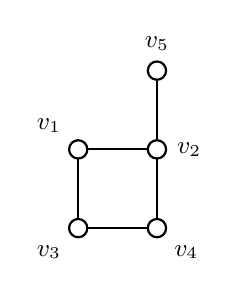
\begin{tikzpicture}[thick,scale=1]
   \tikzset{node/.style 2 args={draw, circle,draw=black,scale=0.7, label=#1:{\large #2}}};
   \node[node={135}{\small $v_1$} ] (0) at (0,0) {}; 
\node[node={0}{\small $v_2$} ] (1) at (1,0) {};
\node[node={225}{\small $v_3$} ] (2) at (0,-1) {};
\node[node={315}{\small $v_4$} ] (3) at (1,-1) {};
\node[node={90}{\small $v_5$} ] (4) at (1,1) {};

\draw (0) -- (1);
\draw (0) -- (2);
\draw (2) -- (3);
\draw (3) -- (1);
\draw (1) -- (4);
   
\end{tikzpicture}
\end{minipage}
\begin{minipage}[c]{0.05\linewidth}
$\Rightarrow$
\end{minipage}
\begin{minipage}[c]{0.7\linewidth}
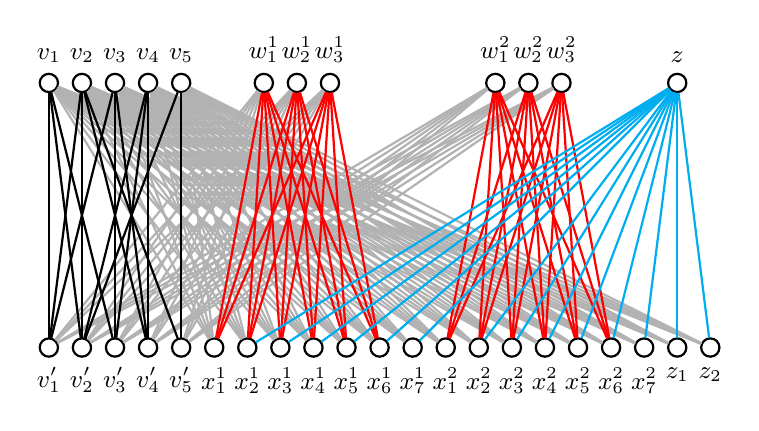
\begin{tikzpicture}[thick,scale=0.42]
   \tikzset{node/.style 2 args={draw, circle,draw=black,scale=0.7, label=#1:{\large #2}}};

\node[node={90}{\small $v_1$} ] (0) at (0,0) {}; 
\node[node={90}{\small $v_2$} ] (1) at (1,0) {};
\node[node={90}{\small $v_3$} ] (2) at (2,0) {};
\node[node={90}{\small $v_4$} ] (3) at (3,0) {};
\node[node={90}{\small $v_5$} ] (4) at (4,0) {};
\node[node={90}{\small $w_1^1$} ] (5) at (6.5,0) {};
\node[node={90}{\small $w^1_2$} ] (6) at (7.5,0) {};
\node[node={90}{\small $w^1_3$} ] (7) at (8.5,0) {};
\node[node={90}{\small $w^2_1$} ] (8) at (13.5,0) {};
\node[node={90}{\small $w^2_2$} ] (9) at (14.5,0) {};
\node[node={90}{\small $w^2_3$} ] (10) at (15.5,0) {};
\node[node={90}{\small $z$} ] (11) at (19,0) {};

\node[node={270}{\small $v'_1$} ] (12) at (0,-8) {};
\node[node={270}{\small $v'_2$} ] (13) at (1,-8) {};
\node[node={270}{\small $v'_3$} ] (14) at (2,-8) {};
\node[node={270}{\small $v'_4$} ] (15) at (3,-8) {};
\node[node={270}{\small $v'_5$} ] (16) at (4,-8) {};

\foreach \i in {1,...,7}{
        \node[node={270}{\small $x^{1}_{\i}$} ] (a\i) at (4 + \i ,-8) {};}

\foreach \i in {1,...,7}{
        \node[node={270}{\small $x^{2}_{\i}$} ] (b\i) at (4 + \i + 7,-8) {};}

\node[node={270}{\small $z_1$} ] (31) at (19,-8) {};
\node[node={270}{\small $z_2$} ] (32) at (20,-8) {};
%-
%Ec--------------------------

\foreach \i in {0,...,4}{
    \foreach \j in {1,...,7}{
        \draw (\i) edge[gray!60] (a\j);
    }
}

\foreach \i in {0,...,4}{
    \foreach \j in {1,...,7}{
        \draw (\i) edge[gray!60] (b\j);
    }
}

\foreach \j in {0,...,4}{
    \draw (\j) edge[gray!60] (31);
    \draw (\j) edge[gray!60] (32);
}

\foreach \i in {12,...,16}{
    \foreach \j in {5,...,10}{
        \draw (\i) edge[gray!60] (\j);
    }
}

%Ewx-----------------------------

\foreach \i in {5,6,7}{
    \foreach \j in {1,...,6}{
        \draw (\i) edge[red] (a\j);
    }
}

\foreach \i in {8,9,10}{
    \foreach \j in {1,...,6}{
        \draw (\i) edge[red] (b\j);
    }
}

%Ed----------------------

\draw (0) -- (12);
\draw (0) -- (13);
\draw (0) -- (14);

\draw (1) -- (12);
\draw (1) -- (13);
\draw (1) -- (15);
\draw (1) -- (16);

\draw (2) -- (12);
\draw (2) -- (14);
\draw (2) -- (15);

\draw (3) -- (13);
\draw (3) -- (14);
\draw (3) -- (15);

\draw (4) -- (13);
\draw (4) -- (16);

%Ez-----------------

\foreach \j in {2,...,7}{
    \draw (11) edge[cyan] (a\j);
}
\foreach \j in {2,...,7}{
    \draw (11) edge[cyan] (b\j);
}
\draw (31) edge[cyan] (11);
\draw (32) edge[cyan] (11);

\end{tikzpicture}
\end{minipage}
\caption{A graph $G$, instance of \textsc{Dominating Set} and the  bipartite graph $G'$ obtained from $G$, for $k=2$ and $n=5$.}
\end{center}
\end{figure}\label{bipartitefigure}
\begin{theorem} \label{bipartite}
\DGP~parameterized by (an upper bound on) the number of clusters in an optimal solution is  W[2]-hard on dense bipartite graphs. 
\end{theorem}
\begin{proof}

We give a reduction from {\sc Dominating Set}. Given a graph $G=(V,E)$ with $V=\{v_1,\dots,v_n\}$ and an integer $k$ as instance of {\sc Dominating Set}, we construct a bipartite graph $G'=(V_1,V_2,E')$ as input for \DGP~as follows:
\begin{itemize}
\item $V_1= V\cup \{w_i^j\colon 1\leq i\leq n-k, \  1\leq j\leq k\}\cup\{z\}$
\item $V_2=\{v_1',\dots,v_n'\}\cup\{x_r^j\colon 1\leq r\leq N, \ 1\leq j\leq k\}\cup\{z_i\colon 1\leq i\leq N-n\}$ where $N\in \mathbb{N}$ is chosen as follows.
Let $c\in \mathbb N$ be the smallest integer such that  $c(n-k+1)-1 > n$ (note that $1\leq c\leq n$) and define $N=c(n-k+1)-1$. For this choice of $N$ it follows that the greatest common divisor of $N$ and $n-k+1$ is 1, and $n<N\leq 2n$.
\item $E'=E_d\cup E_{wx}\cup E_c  \cup E_z$ with

$E_d=\{\{v_i,v_j'\}\colon \{v_i,v_j\}\in E\}\cup \{\{v_i,v_i'\}\colon 1\leq i\leq n \}$,\\
$E_{wx}=\{\{w_i^j,x_r^j\}\colon 1\leq i\leq n-k, \ 1\leq r\leq N-1, 1\leq j\leq k \}$, \\
$E_c=\{\{w_i^j,v_s'\}\colon 1\leq i\leq n-k, 1\leq j\leq k,\ 1\leq s\leq n\}\cup\{\{v_s,x_r^j\}\colon 1\leq s\leq n, \ 1\leq r\leq N, \ 1\leq j\leq k\}$ and \\ $E_z=\{\{z,z_j\}\colon 1\leq j\leq N-n\} \cup \{\{z,x^j_r\} : 2\leq r\leq N, 1\leq j\leq k \} \cup\{\{v_i,z_j\}\colon 1\leq i\leq n, \  1\leq j\leq N-n \}$
\end{itemize}
Notice that  $G'$ is a bipartite graph with $|V_1|=n+1+ k(n-k)$ and  $|V_2|= (k+1)N$.

We show that there exits a dominating set of cardinality at most $k$ in $G$ if and only if there exists a partition  $\mathcal{P}$ of $G'$ with  $d(\mathcal{P})=(k+1)d(G_{n-k+1,N})$.


Suppose there exists a dominating set $D$ in $G$ with $|D|=k$.
Let $D=\{v_{i_1},\dots,v_{i_k}\}$  and $N'(v_{i_j})=N_G[v_{i_j}]\setminus (D\cup N_G(\{v_{i_1},\dots, v_{i_{j-1}}\})$. Define the partition $\mathcal{P}=\{P_1,\dots,P_{k+1}\}$ by:\\ $P_j=\{v_{i_j}\}\cup \{v_r'\colon v_r \in N'(v_{i_j})\} \cup \{w_r^j\colon 1\leq r \leq n-k\} \cup\{x_r^j\colon 1\leq r\leq N-|N'(v_{i_j})| \}$ for $1\leq j\leq k $ and $P_{k+1}=V_1\cup V_2\setminus (\cup_{j=1}^k P_j)$.
It is not hard to see that the vertices in $P_j$ induce a complete bipartite graph $G_{n-k+1,N}$ for each $j$. Thus $d(\mathcal{P})=(k+1)d(G_{n-k+1,N})$.



Conversely, let $\mathcal{P}$ be a partition of $G'$ of density $(k+1)d(G_{n-k+1,N})$.
Thus, Corollary~\ref{bipar_cond} implies that the vertices for each set $P\in \mathcal{P}$ induce a complete bipartite graph $G_{r,s}$ such that $\frac rs=\frac{|V_1|}{|V_2|}=\frac{k(n-k)+n+1}{(k+1)N}=\frac{n-k+1}{N}$. Since the greatest common divisor of $n-k+1$ and $N$ is one, this yields $r\geq n-k+1$ and $s\geq N$ and especially $\mathcal{P}$ can contain at most $k+1$ sets. 

For all $w_i^j$ and $w_{\ell}^{t}$, if $j \neq t$, $w_i^j$ and $w_{\ell}^{t}$ have $n$ common neighbours, and $n < N$ then there is no part $P\in \mathcal{P}$ such that $w_i^j, w_{\ell}^{t} \in P$. Moreover, for all $i,j$, $w_i^j$ and $z$ have $N-1$ common neighbours so they cannot be in the same $P\in \mathcal{P}$. Hence, there are exactly $k+1$ parts in $\mathcal{P}$ that are complete bipartite graphs $G_{n-k+1,N}$.


For all $1 \leq j \leq k$,  denote by $P_j$ the set containing the vertices $w^j_i$ for all $1 \leq i \leq n-k$ and $P_z$ the part containing $z$. To reach the cardinality exactly $n-k+1$, $P_j\cap V_1$ has to contain exactly one vertex from $V$ for each $1\leq j\leq k$.
Further, since for any $i$, $v_i'$ is not adjacent to $z$, $V' \subseteq \cup_{j=1}^k P_j$. Moreover, each $P_j$ contains exactly one vertex of $V$.
As each $P \in \mathcal{P}$ induces a complete bipartite graph in $G'$, $D= V \cap  \cup_{j=1}^k P_j$ is a set of size $k$, such that each vertex in $V'$ is adjacent to at least one vertex in $D$, so we deduce that $D$ is dominating set of size $k$ in $G$. 

At last, in case of a yes-instance of \textsc{Dominating Set}, there exists an optimum solution with $k+1$ sets for \textsc{Dense Graph Partition} on $G'$. With parameter $k'=k+1$, the instance $((G',(k+1)d(G_{n-k+1,N})),k')$ describes an fpt-reduction from \textsc{Dominating Set} parameterized by solution size to  \textsc{Max Dense Graph Partition} parameterized by an upper bound on the number of sets, which shows the claimed W[2]-hardness.
% \end{proof}

 
% \begin{theorem}
% \DGP~parameterized by (an upper bound on) the number of clusters in an optimal solution is  W[2]-hard on dense bipartite graphs.
% \end{theorem}
% \begin{proof}
\medskip
We extend the construction of the proof to create from $G'$ a dense bipartite graph $G''=(V'',E'')$ by adding four sets of vertices $V_1^u, V_1^d, V_2^u, V_2^d$ with $|V_1^u|=|V_1^d|=kn|V_1|=kn(k(n-k)+n+1)$  and $|V_2^u|=|V_2^d|=kn|V_2|=knN(k+1)$. Further, we add edges to turn the pairs $(V_1^u, V_2^u)$, $(V_1^d, V_2^d)$, $(V_1^u, V_1)$, and $(V_2^d,V_2)$ each into complete bipartite graphs. Observe that with this construction $G''$ has $|V''|=(2kn+1)(k(n-k)+n+1)+(2kn+1)N(k+1)< 10k^2n^2$  vertices and that all vertices have degree at least $kn|V_1|\geq \frac 12 k^2 n^2\in \Theta(|V''|)$ (Note that the fpt-reduction can solve the instance of {\sc Dominating Set} exactly in the trivial case of $k\geq \frac n2$, so we can assume that $k\leq \frac n2$.).

We claim that there exists a partition $\mathcal{P'}$ of $G''$ with  $d(\mathcal{P'})=(k+1)d(G_{n-k+1,N})+2kn(k+1)d(G_{n-k+1,N})$ if and only if there exists a dominating set of size $k$ for $G$.  Corollary~\ref{bipar_cond} again implies that this density for  $G''$ can only be achieved by a partition into complete bipartite graphs $G_{r,s}$ with $\frac rs=\frac{(2kn+1)(k(n-k)+n+1)}{(2kn+1)N(k+1)}=\frac{n-k+1}{N}$. The vertices in $V_1^d$ are only adjacent to vertices in $V_2^d$, and the vertices in $V_2^u$ are only adjacent to vertices in $V_1^u$. Clustering these in a ratio $\frac rs$ results in clusters containing exactly all newly added vertices, and this can be done with just two sets in total. 
What remains is to cluster the graph $G'$ into complete bipartite graphs $G_{r,s}$ such that $\frac rs=\frac{|V_1|}{|V_2|}=\frac{k(n-k)+n+1}{(k+1)N}=\frac{n-k+1}{N}$ as before.

At last, in case of a yes-instance of \textsc{Dominating Set}, there exists an optimum solution with $k+3$ sets for \textsc{Dense Graph Partition} on $G''$. With parameter $k'=k+3$, the instance $((G'',(2kn+1)(k+1)d(G_{n-k+1,N})),k')$ describes an fpt-reduction from \textsc{Dominating Set} parameterized by solution size to  \textsc{Max Dense Graph Partition} parameterized by an upper bound on the number of sets, which shows the claimed W[2]-hardness
\end{proof}






 
\section{Cubic Graphs }\label{sec4}
\label{sec:cubicDense}

We show that the problem \DGP~is NP-complete even for cubic graphs by giving a reduction from \textsc{Exact Cover By 3-Sets} where each element appears in exactly 3 sets, denoted \textsc{Restricted Exact Cover By 3-Sets},  known to be NP-hard by~\cite{Gonzalez85}.

 
\defprob{Restricted Exact Cover By 3-Sets (RX3C)}{A set $X$ of elements with $|X| = 3q$ and a collection $C$ of 3-element subsets of $X$ where each element appears in exactly 3 sets.}{Does $C$ contain an exact cover for $X$, i.e. a subcollection $C' \subseteq C$ such that every element occurs in exactly one member of $C'$ ?}

\noindent
Before describing the reduction, we give useful notions for utility.
%\noindent


\begin{definition}
For $S \subseteq V$, the utility of a vertex  $v \in S$ is defined by  $u_S(v) = \frac{d(S)}{|S|}$, and the utility of $S$ is defined by $u(S)=u_S(v)$ for any $v \in S$. For a partition $\mathcal{P}= \{ V_1, \ldots, V_k\}$, the utility of a vertex $v$ in $\mathcal{P}$ is defined by  $u_{\mathcal{P}}(v)=u_{V_i}(v)$ with $i$ such that $v\in V_i$. 
\end{definition}

 
Considering these definitions, we can remark that:
\begin{itemize} 
\item  For any subset $S \subseteq V$, and $v,w \in S $, $u_S(v)=u_S(w)$.
\item If $S=\{v\}$ then $u_S(v)=0$.
\item  For any partition $\mathcal{P}$ of $G$, $\sum\limits_{V_i \in \mathcal{P}}d(V_i) = \sum\limits_{v \in V}u_{\mathcal{P}}(v)$. 
\end{itemize}
 
  
\noindent
The following definition gives the construction to reduce \textsc{RX3C} to \DGP.
%We first describe a polynomial-time reduction from RX3C to \DGP~and then prove a lemma allowing us to prove the NP-completeness of \DGP~on cubic graphs. 


\begin{figure}
\begin{minipage}[c]{0.49\linewidth}
    \centering
   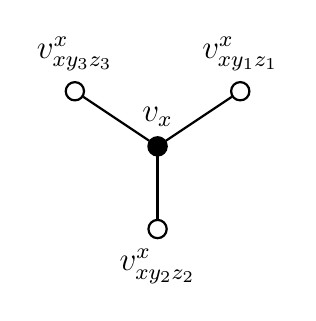
\begin{tikzpicture}[thick,scale=0.35]
   \tikzset{node/.style 2 args={draw, circle,draw=black,scale=0.7, label=#1:{\large #2}}};
   


\node[node={90}{$v_x$},fill ] (1) at (0,0) {};
\node[node={90}{$v_{xy_1z_1}^x$} ] (2) at (3,2) {} edge (1);
\node[node={270}{$v_{xy_2z_2}^x$} ] (3) at (0,-3) {} edge (1);
\node[node={90}{$v_{xy_3z_3}^x$} ] (4) at (-3,2) {} edge (1) ;


\end{tikzpicture}
\caption{Subgraph containing one vertex of type 1, $v_x$, and its neighbors in $G$}
\label{t1}
\end{minipage}
\begin{minipage}[c]{0.49\linewidth}
    \centering
   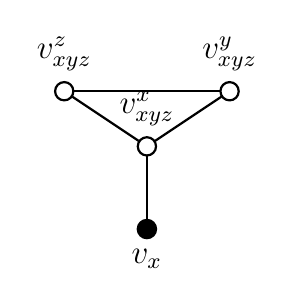
\begin{tikzpicture}[thick,scale=0.35]
   \tikzset{node/.style 2 args={draw, circle,draw=black,scale=0.7, label=#1:{\large #2}}};

\node[node={90}{$v_{xyz}^x$} ] (1) at (0,0) {};
\node[node={90}{$v_{xyz}^y$} ] (2) at (3,2) {} edge (1);
\node[node={270}{$v_x$},fill ] (3) at (0,-3) {} edge (1);
\node[node={90}{$v_{xyz}^z$} ] (4) at (-3,2) {} edge (1) edge(2) ;


\end{tikzpicture}
\caption{Subgraph containing one vertex of type 1, $v_x$, and three of type 2}
\label{t2}
\end{minipage}

\end{figure}

 
\begin{definition}\label{construction}
Let $I=(X,C)$ be an instance of $RX3C$. We define the construction $\sigma$ transforming the instance $I$ into the graph $G:= \sigma(I)$ where  $G=(V,E)$  as follows: 

\begin{itemize}
    \item for each element $x \in X$, we add the vertex $v_x$ in $V$ (called vertices  of type 1 or black vertices).
    \item for each subset of the collection $\{x,y,z\} \in C$, we add the vertices $v_{xyz}^x$, $v_{xyz}^y$, $v_{xyz}^z$ in $V$ (called vertices  of type 2 or white vertices).
    \item we add the edges $\{v_{xyz}^x,v_{xyz}^y\}$, $\{v_{xyz}^x,v_{xyz}^z\}$ and $\{v_{xyz}^y,v_{xyz}^z\}$ to $E$  
    \item we add the edges $\{v_{xyz}^x,v_x\}$, $\{v_{xyz}^y,v_y\}$ and $\{v_{xyz}^z,v_z\}$ to $E$ 
\end{itemize}

\noindent
\normalfont{Notice that $G$ is a cubic graph on $|X|$ vertices of type 1, $3|X|$ vertices of type 2. 
%and contains $6|X|$ edges.
}
\end{definition}



\noindent
Case distinction on the subgraphs in $\sigma(I)$ shows:

\begin{lemma}\label{casescubic}
For any subset $S\subseteq V$ of the vertices of the graph $\sigma(I)$, the only subgraphs $G[S]$ with $u(S) \geq \frac{1}{4}$ are:
\begin{itemize}
    \item a triangle where all the vertices are of type 2 and then $u(S) = \frac{1}{3}$.
    \item a matching between two  type 2 vertices or between  two vertices of different types and then  $u(S) =  \frac{1}{4}$.
    \item the subgraph described in Figure \ref{t2} and then $u(S) =  \frac{1}{4}$.
\end{itemize} 
\label{lem:utiliteG}
\end{lemma}

\begin{proof}
Let $S\subseteq V$ such that $u(S) \geq \frac{1}{4}$. We show in the following that there are exactly three possible  subgraphs $G[S]$ such that  $u(S) \geq \frac{1}{4}$. 
First, observe that by its construction $G$ does not contain $C_4$ as subgraph, since there are no two vertices $u,v\in V$ that have more than one common neighbor. Note that this also implies that $G$ is diamond-free.

As $G$ is cubic, $|E(G[S])| \leq \frac{3}{2}|S|$ and  so $d(S) \leq \frac{3}{2}|S|\cdot \frac{1}{|S|} = \frac{3}{2}$. Since $\frac{1}{4} \leq u(S) \leq \frac{3}{2|S|}$  then $|S| \leq 6$. We study the five following cases :
\begin{itemize}
    \item Case $|S| = 6$ : Since $u(S)= \frac{|E(S)|}{6^2}  \geq \frac{1}{4}$,  we have $|E(S)| \geq 9$. Since $G[S]$ cannot be cubic ($G$ is connected and $|V| > 6$), a subgraph with $|S|=6$ and $|E(S)| \geq 9$ does not exist.
    \item Case $|S| = 5$ : Since $u(S)= \frac{|E(S)|}{5^2} \geq \frac{1}{4}$,  we have $|E(S)| \geq 7$. Assuming such a subgraph with $|S| = 5$ and $|E(S)| \geq 7$, $G[S]$ must contain a diamond or a clique of size 4. Since $G=\sigma(I)$ is diamond-free and $G$ is cubic, such a  subgraph does not exist.
    \item Case $|S| = 4$ : Since $u(S)= \frac{|E(S)|}{4^2} \geq \frac{1}{4}$,  we have $|E(S)| \geq 4$.    Since $G$ is diamond-free, $G$ is not a $K_4$ or a $C_4$  the only possibility for $G[S]$ is the subgraph described in Figure \ref{t2}.
    \item Case $|S| = 3$ : Since $u(S) = \frac{|E(S)|}{3^2} \geq \frac{1}{4}$,  we have $|E(S)| \geq 3$ and thus $S$ is a triangle where all the vertices are of type 2 and $u(S) = \frac{1}{3}$.
    \item Case $|S| = 2$ : Since $u(S) = \frac{|E(S)|}{2^2}  \geq  \frac{1}{4}$, we have $|E(S)| \geq 1$ and thus $S$ is a matching between two  type 2 vertices or between two vertices of different types and $u(S) = \frac{1}{4}$.
\end{itemize}
\end{proof}


\begin{remark}
For any subset $S\subseteq V$ of the vertices of the graph $\sigma(I)$, if $v$ is of type 2 then $u_S(v) \leq \frac{1}{3}$, otherwise $u_S(v) \leq \frac{1}{4}$.
\end{remark}
With these observations about the construction of $\sigma(I)$, it can be shown that $I=(X,C)$ is a yes-instance of RX3C if and only if $I'=(\sigma(I),d)$ is a yes-instance of \DGP{} which yields the following.
\begin{theorem}\label{cubichardness}
\DGP~is NP-complete on cubic graphs.
\end{theorem}

\begin{proof}
Let $I=(X,C)$ be an instance of RX3C and consider the following instance $I'$ of \DGP{} on the graph $G=\sigma(I)$ and $d=\frac{7|X|}{6}$. 
We claim that $I=(X,C)$ is a yes-instance of RX3C if and only if $I'=(G,d)$ is a yes-instance of \DGP. 

\medskip
  Let $C' \subseteq C$ be an exact cover for $X$ of size $\frac{|X|}{3}$. Consider the following partition $\mathcal{P}$ with $\frac{5|X|}{3}$ parts : for any $c \in C'$, $c=\{x,y,z\}$, we define three parts of size 2 $\{v_x, v_{xyz}^x\}$, $\{v_y, v_{xyz}^y\}$, $\{v_z, v_{xyz}^z\}$ and for any $c \notin C'$, $c=\{x,y,z\}$, we define the following part of size 3  $\{v_{xyz}^x, v_{xyz}^y, v_{xyz}^z\}$. Since $C'$ is an exact cover, $\mathcal{P}$ is a partition and its density is $\frac{3}{2}\cdot\frac{|X|}{3} + \frac{2}{3}|X| = \frac{7}{6}|X|$.
\medskip

Let $\mathcal{P'}$ be a partition of $G$ of density $d(\mathcal{P'})=\frac{7}{6}|X|$. Firstly, we show  that $\mathcal{P'}$ has necessarily the following shape: $\frac{2|X|}{3}$ parts of size 3 containing only vertices of type 2 forming a triangle in $G$ and $|X|$ parts of size 2 containing one vertex of type 1 and one of type 2 adjacent in $G$ (see Figures \ref{t1} and \ref{t2}). From Remark~\ref{remarkconnexe}, we can consider that   for every part $P_i \in \mathcal{P'}$, $G[P_i]$ is connected.  

We  prove in the following  that since $d(\mathcal{P'})=\frac{7|X|}{6}$ then there are at least $\frac{2|X|}{3}$ parts in $\mathcal{P'}$ corresponding to triangles in $G$.  
Assume by contradiction that $\mathcal{P'}$ has $\frac{2|X|}{3} - \ell $ triangles, with $\ell > 0$. Since $G$ has $4|X|$ vertices, there are $2|X|+ 3 \ell$ vertices that do not belong to a part in $\mathcal{P'}$ that corresponds to a triangle in $G$.  By Lemma \ref{lem:utiliteG} the utility of these last vertices  is smaller than or equal to $\frac{1}{4}$. Then the density of $\mathcal{P'}$ is 
\[
    d(\mathcal{P}') \leq   \frac{2|X|}{3} - \ell + (2|X|+ 3 \ell) \cdot\frac{1}{4}  \leq  \frac{7|X|}{6} - \frac{\ell}{4}  < \frac{7|X|}{6}
\]
This contradicts the choice of  $\mathcal{P'}$ such that   $d(\mathcal{P'})=\frac{7|X|}{6}$, hence there are at least $\frac{2|X|}{3}$ triangles in $\mathcal{P'}$.

Now, we will prove that there are at most $\frac{2|X|}{3}$ parts in $\mathcal{P'}$ corresponding to triangles in $G$. Assume by contradiction that $\mathcal{P'}$ has $\frac{2|X|}{3} + \ell$ triangles, with $\ell > 0$. Since there are $3|X|$ vertices of type 2 and among these vertices $3\cdot(\frac{2|X|}{3} + \ell)$   belong to a triangle then $|X|-3 \ell$ vertices of type 2 do not belong to a triangle. But each neighbour of a vertex $v_x$ of type 1 is of type 2, so if  the utility of $v_x$ is positive, then there exists a vertex of type 2, $v^x_{xyz}$, neighbour of $v_x$,  that is in the same part as $v_x$ and $v^x_{xyz}$  does not belong to a triangle. Moreover, as all type 1 vertices have no common neighbours, for each type 1 vertex with positive utility, there is a type 2 vertex that is not in a triangle. Since there are at most $|X|-3 \ell$ type 2 vertices that do not belong to a triangle, there are at most $|X|-3 \ell$ type 1 vertices with positive utility.  Then the density of $\mathcal{P'}$ is at most

 

\[
    d(\mathcal{P'}) \leq \frac{2|X|}{3}+ \ell + \frac{|X| - 3 \ell}{4} + \frac{|X| - 3 \ell}{4} \leq \frac{7|X|}{6} - \frac{\ell}{2} < \frac{7|X|}{6}
\]
This contradicts   the choice of  $\mathcal{P'}$ such that  $d(\mathcal{P'})=\frac{7|X|}{6}$,  and then there are exactly $\frac{2|X|}{3}$ triangles in $\mathcal{P'}$.

We will show now that  $d(\mathcal{P'}) = \frac{7|X|}{6}$ implies that all type 1 vertices are in a part that is a matching with a type 2 vertex. There are $|X|$ type 1 vertices and $|X|$ type 2 vertices that are not in some triangle in $\mathcal{P'}$.  Since there are exactly  $\frac{2|X|}{3}$ parts in $\mathcal{P'}$ forming a triangle and the utility of each other vertex is smaller than or equal to $\frac{1}{4}$, to reach a density of $\frac{7|X|}{6}$ it is necessary that each of the $2|X|$ vertices outside the parts that are triangles  has a utility of exactly $\frac{1}{4}$.  To reach this utility, by Lemma \ref{lem:utiliteG} there are two possibilities, the graph described in Figure \ref{t2} and an edge. Since there are exactly $|X|$ vertices of type 1  and $|X|$  vertices of type 2  outside the triangles in $\mathcal{P'}$, and vertices of type 1 only have neighbors of type 2, the only possibility for all these vertices to have utility $\frac{1}{4}$ is if each type 1 vertex is matched with one type 2 vertex.
%For the first, there are three vertices of type 2 for one of type 1 so we cannot reach $\frac{7|X|}{6}$ so all type 1 vertices are in a matching with a type 2 vertex.  Finally, observe that for every $\{x,y,z\}$ in $C$, if $v^x_{xyz}$ is in a matching with $v_x$, then $v^y_{xyz}$ is in a matching with $v_y$ and  $v^z_{xyz}$ is in a matching with $v_z$. Otherwise, $v^y_{xyz}$ is   in a matching with $v^z_{xyz}$, which is impossible since there are $|X|$ vertices type 1  and $|X|$  vertices type 2  outside the triangles in $\mathcal{P'}$. 

Consider now the following subcollection $C''\subseteq C$: for each triple $v^x_{xyz}$,$v^y_{xyz}$,$v^z_{xyz}$ that does not belong to a triangle, we add the set $\{x,y,z\}$ to $C''$. The subcollection $C''$ is a cover since each type 1 vertex is a neighbour of one of these vertices and it is an exact cover  since there are exactly  $\frac{|X|}{3}$ 3-element subsets that do not belong to a triangle.
\end{proof}
 
 

In the following we give a polynomial time  $\frac{4}{3}$-approximation for \MDGP{} on cubic graphs. We start with some preliminary results. 
\begin{lemma}
\label{lem:utilPasTriDia}
Let $G=(V,E)$ be a cubic graph. Let $\mathcal{P}$ any partition of $V$. 
%Let $P \in \mathcal{P}$ be the part that contains $v$. 
If a part $P$ of $\mathcal P$ is not a triangle or a diamond, then $u_\mathcal{P}(v) \leq \frac{1}{4}$ for any $v\in P$.
\end{lemma}
\begin{proof}
Since the graph is cubic, $d(P) \leq \frac{3|P|}{2|P|} = \frac{3}{2}$. Then $u_{\mathcal{P}}(v) \leq \frac{3}{2|P|}$. If $|P| \geq 6$, $u_{\mathcal{P}}(v) \leq \frac{3}{2 \cdot 6} = \frac{1}{4}$. If $|P| < 6$ and since $P$ is not a triangle or a diamond, by exhaustive search,  $u_{\mathcal{P}}(v)$ is maximised when $P$ is a matching and its value is $\frac{1}{4}$.
\end{proof}
\begin{lemma}
\label{lem:UtilMatchCubique}
Let $G$ be a cubic graph. For every vertex $v$ of $G$ that does not belong to a triangle of $G$, $u_{\mathcal{P}}(v) \leq \frac{1}{4}$ for any partition $\mathcal{P}$ of $V$.
 \end{lemma}
 \begin{proof}
 The lemma is a direct consequence of \autoref{lem:utilPasTriDia}.
 \end{proof}

\begin{lemma}
\label{lem:UtilDiamCubique}
Let $G$ be a cubic graph with at least one diamond. Let $v_1,v_2,v_3,v_4$ be a diamond in $G$ where $v_1$ and $v_3$ are the induced degree two vertices. Then $u_{\mathcal{P}}(v_1) + u_{\mathcal{P}}(v_2) + u_{\mathcal{P}}(v_3) + u_{\mathcal{P}}(v_4) \leq \frac{5}{4}$ for any partition $\mathcal{P}$.
\end{lemma}


\begin{figure}[ht]
    \centering
    \begin{minipage}[c]{0.3\textwidth}
        \centering
        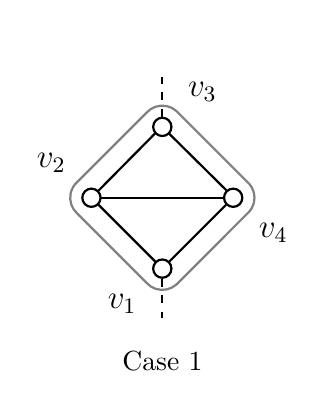
\begin{tikzpicture}[thick, label distance=0.15cm,scale=0.9]
                     \tikzset{node/.style 2 args={draw, circle,draw=black,scale=0.7, label=#1:{\large #2}}};
            \node[node={225}{$v_1$} ] (1) at (0,0) {};
            \node[node={135}{$v_2$}] (2) at (-1,1) {};
            \node[node={45}{$v_3$} ] (3) at (0,2) {};
            \node[node={315}{$v_4$} ] (4) at (1,1) {};
            
            \node (n1) at (0,-1) {};
            \node (n3) at (0,3) {};
            
            \draw[dashed] (1)--(n1);
            \draw[dashed] (3)--(n3);
            
            \draw[] (1)--(2);
            \draw[] (2)--(3);
            \draw[] (3)--(4);
            \draw[] (4)--(1);
            \draw[] (2)--(4);
            
            \fill[color=white] (-1,-1.4) rectangle (1,-0.7);
            
            \fill[color=white] (-1,3.4) rectangle (1,2.7);
            
            \draw[gray] \convexpath{1,2,3,4}{0.3 cm};
            
            \node (n1) at (0,-1.3) {Case 1};
        \end{tikzpicture}
    \end{minipage}
    \begin{minipage}[c]{0.3\textwidth}
        \centering
        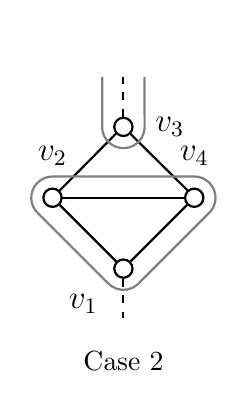
\begin{tikzpicture}[thick, label distance=0.15cm,scale=0.9]
            \tikzset{node/.style 2 args={draw, circle,draw=black,scale=0.7, label=#1:{\large #2}}};
            \node[node={225}{$v_1$} ] (1) at (0,0) {};
            \node[node={90}{$v_2$}] (2) at (-1,1) {};
            \node[node={0}{$v_3$} ] (3) at (0,2) {};
            \node[node={90}{$v_4$} ] (4) at (1,1) {};
            
            \node (n1) at (0,-1) {};
            \node (n3) at (0,3) {};
            
            \draw[dashed] (1)--(n1);
            \draw[dashed] (3)--(n3);
            
            \draw[] (1)--(2);
            \draw[] (2)--(3);
            \draw[] (3)--(4);
            \draw[] (4)--(1);
            \draw[] (2)--(4);
            
            \fill[color=white] (-1,-1.4) rectangle (1,-0.7);
            
            \draw[gray] \convexpath{3,n3}{0.3 cm};
            \fill[color=white] (-1,3.4) rectangle (1,2.7);
            
            \draw[gray] \convexpath{1,2,4}{0.3 cm};
            \node (n1) at (0,-1.3) {Case 2};
        \end{tikzpicture}
    \end{minipage}
    \commente{
    \begin{minipage}[c]{0.3\textwidth}
        \centering
        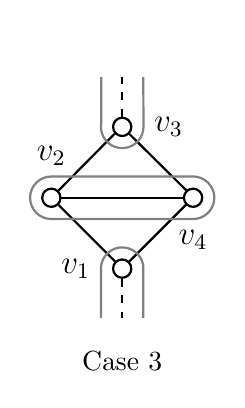
\begin{tikzpicture}[thick, label distance=0.15cm,scale=0.9]
            \tikzset{node/.style 2 args={draw, circle,draw=black,scale=0.7, label=#1:{\large #2}}};
            \node[node={180}{$v_1$} ] (1) at (0,0) {};
            \node[node={90}{$v_2$}] (2) at (-1,1) {};
            \node[node={0}{$v_3$} ] (3) at (0,2) {};
            \node[node={270}{$v_4$} ] (4) at (1,1) {};
            
            \node (n1) at (0,-1) {};
            \node (n3) at (0,3) {};
            
            \draw[dashed] (1)--(n1);
            \draw[dashed] (3)--(n3);
            
            \draw[] (1)--(2);
            \draw[] (2)--(3);
            \draw[] (3)--(4);
            \draw[] (4)--(1);
            \draw[] (2)--(4);
            
            \draw[gray] \convexpath{1,n1}{0.3 cm};
            \fill[color=white] (-1,-1.4) rectangle (1,-0.7);
            
            \draw[gray] \convexpath{3,n3}{0.3 cm};
            \fill[color=white] (-1,3.4) rectangle (1,2.7);
            
            \draw[gray] \convexpath{2,4}{0.3 cm};
            \node (n1) at (0,-1.3) {Case 3};
        \end{tikzpicture}
    \end{minipage}
    }
        \caption{Different cases of \autoref{lem:UtilDiamCubique}}\label{fig:utilDiamants}
  
\end{figure}

\begin{proof}
Let $\mathcal{P}$ be any partition of $V$. Let $P_1 \in \mathcal{P}$ (resp. $P_2$, $P_3$ and $P_4$) be the part that contains $v_1$ (resp. $v_2$, $v_3$ and $v_4$). We distinguish several cases.
\noindent
\textbf{Case 1:} The four   vertices $v_i$ are in the same part and this part is a diamond. Then $d(P_1) = \frac{5}{4}$ and thus $u_{\mathcal{P}}(v_1) + u_{\mathcal{P}}(v_2) + u_{\mathcal{P}}(v_3) + u_{\mathcal{P}}(v_4) = \frac{5}{4}$.
 
\noindent
\textbf{Case 2:} Three among the four vertices of the diamond forming a triangle are in the same part. The other one cannot belong to a part that is a triangle or an diamond. Then, by \autoref{lem:utilPasTriDia}, $u_{\mathcal{P}}(v_1) + u_{\mathcal{P}}(v_2) + u_{\mathcal{P}}(v_3) + u_{\mathcal{P}}(v_4) \leq 1 + \frac{1}{4} = \frac{5}{4}$.
 

\noindent
\textbf{Case 3:} $P_1$, $P_2$, $P_3$ and $P_4$ are not triangles or diamonds then, by \autoref{lem:utilPasTriDia}, for all $v \in \cup_{i \leq 4} P_i$, $u_{\mathcal{P}}(v) \leq \frac{1}{4}$. We conclude that $u_{\mathcal{P}}(v_1) + u_{\mathcal{P}}(v_2) + u_{\mathcal{P}}(v_3) + u_{\mathcal{P}}(v_4) \leq 1$.
\end{proof}



\begin{lemma}
\label{lem:UtilTriangleCubique}
Let $G$ be a cubic graph and $v$ a vertex of $G$. Then $u_{\mathcal{P}}(v) \leq \frac{1}{3}$ in any partition $\mathcal{P}$ of $V$.
\end{lemma}

\begin{proof}
Let $P$ be the part of $\mathcal{P}$ that contains $v$. Using the same reasoning as in the proof of \autoref{lem:utilPasTriDia}, we deduce that if $|P| \geq 5$ then $u_{\mathcal{P}}(v) < \frac{1}{3}$. If $|P| < 5$, by exhaustive search, $u_{\mathcal{P}}(v)$ is maximised when  $P$ is a   triangle  and in this case $u_{\mathcal{P}}(v) = \frac{1}{3}$.
\end{proof}

\begin{lemma}
\label{lem:ApproxBorneCubique}
Let $G$ be a cubic graph on $n$ vertices and let $D$ be the set of diamonds in $G$ and $T$ the set of triangles in $G$  that do not belong to a diamond. For any partition $\mathcal{P}$, $d(\mathcal{P}) \leq \frac{5}{4}|D| + |T| + \frac{1}{4}(n - 3|T| - 4|D|)$.
\end{lemma}
\begin{proof}
By \autoref{lem:UtilDiamCubique}, we know that the sum of the utilities of the vertices constituting a diamond is at most $\frac{5}{4}$. By \autoref{lem:UtilTriangleCubique}, we deduce that the sum of the utilities of the vertices constituting a triangle is at most $3 \cdot \frac{1}{3} = 1$. The other vertices that do not belong to a triangle or a diamond have a utility of at most $\frac{1}{4}$ (\autoref{lem:UtilMatchCubique}). We deduce that $d(G) \leq \frac{5}{4}|D| + |T| + \frac{1}{4}(n - 3|T| - 4|D|)$.
\end{proof}

\begin{theorem}
\MDGP{} is polynomial time $\frac{4}{3}$-approximable on cubic graphs.
\end{theorem}
\begin{proof}
	Let $I=G$ be a cubic graph, instance of \MDGP{}. Let~$D$ be the set of all diamonds in $G$, and $T$ the set of all triangles  that do not belong to a diamond.
	Diamonds (resp. triangles) can be found in polynomial time simply by enumerating all 4-tuples (resp. 3-tuples) of vertices and checking if they induce a diamond (resp. triangle) as subgraph. %Moreover $\cup_{D_i \in D} D_i \cap \cup_{T_i \in T} T_i = \emptyset$. 
	Let $G'$   be the graph obtained from $G$ after removing the vertices of $D$ and $T$. Let $M$ be the set of edges  that constitute a maximal matching of $G'$. Let $G''$ be the graph obtained from $G'$ after removing the vertices of $M$. Since $M$ is a maximal matching, $G''$ is an independent set. Since $G$ is cubic, the maximum size of an independent set is $\frac{|V|}{4}$, thus $|V(G'')| \leq \frac{|V|}{4}$.
	 Consider the partition $\mathcal{P} = D \cup T \cup M \cup V(G'')$ in the sense that $\mathcal{P}$ contains a set for each diamond in $D$, one set for each triangle in $T$, one set for each edge in the matching $M$ and one set for each vertex in $V(G'')$.
	 %where  each part contains a diamond from $D$, or a triangle from $T$ or an edge from $M$, and the independent set $V(G'')$.
	  Then $d(\mathcal{P}) = \frac{5}{4}|D| + |T| + \frac{1}{4} |M| \geq \frac{5}{4}|D| + |T| + \frac{1}{4}(n - 3|T| - 4|D| - \frac{n}{4})$. By \autoref{lem:ApproxBorneCubique} we know that $opt(I) \leq \frac{5}{4}|D| + |T| + \frac{1}{4}(n - 3|T| - 4|D|)$. Then $\frac{opt(I)}{d(\mathcal{P})} \leq \frac{\frac{5}{4}|D| + |T| + \frac{1}{4}(n - 3|T| - 4|D|)}{\frac{5}{4}|D| + |T| + \frac{1}{4}(n - 3|T| - 4|D| - \frac{n}{4})} = \frac{\frac{1}{4}|D| + \frac{1}{4}|T| + \frac{n}{4}}{\frac{1}{4}|D| + \frac{1}{4}|T| + \frac{3n}{16}} = 1+\frac{{n}}{4|D|+4|T|+{3n}}$. This function is maximized when $|D| = |T| = 0$. Then $\frac{opt(I)}{d(\mathcal{P})} \leq \frac{n}{\frac{3n}{4}} = \frac{4}{3}$.
\end{proof}

 \section{Dense Graphs}\label{sec5}
 \label{sec:densGrapheDensite}
 In this section we consider graphs $G=(V,E)$ on $n$ vertices such that $G$ can be viewed as $G=K_n-H$ where $H$ is a graph of small maximum degree. The edges of $H$ are called \emph{missing edges} in $G$. We first consider graphs $G=(V,E)$ on $n$ vertices such that $\delta(G) \geq n-3$, that is  $G=K_n-H$ where $H$ has $\Delta(H)=2$  and has $q\leq n$ edges and show that \MDGP{} is solvable in polynomial time on these graphs. 
 
 \begin{lemma}\label{threesets}
For any graph $G$ on $n$ vertices such that $\delta(G) \geq n-3$, its density $d(G)$ is greater than or equal to the density of any partition $\mathcal{P}$ of $G$ into $t\geq 3$ parts.
 \end{lemma}
 \begin{proof} 
 The density of $G$ is given by  $d(G)= \frac{\frac{n(n-1)}{2}-q}{n}=\frac{n-1}{2} - \frac{q}{n}$. From Lemma~\ref{lemmacomplete}, among all partitions of $G$ into $t\geq 3$ parts, those where the parts correspond to complete graphs have the largest density.  The density of such a partition in $t$ parts of size $n_1,\ldots,n_t$ is $\frac{n-t}{2}$.  Thus, the density of $G$ is at least as large as the density of this last partition since $t\geq 3$ and $q\leq n$ (note here that a graph with minimum degree $n-3$ has at most $n$ non-edges).
 \end{proof}
 
 
 
Remark that in the proof of the previous lemma when $q=n$ and $t=3$, the density of a partition in 3 parts corresponding to complete subgraphs and the density of the entire graph are the same.    This previous lemma implies that for any graph $G$  such that $\delta(G) \geq n-3$, there exists a partition into one or two parts of maximum density.


 

\begin{lemma}\label{odd}
For any graph $G$ on $n$ vertices such that $\delta(G) \geq n-3$, in any partition into two parts of $G$, the number of missing edges  inside the two parts is at least $o$, where $o$ is the number of odd cycles defined by the missing edges of $G$.
\end{lemma}

\begin{proof}
Let $C$ be and odd cycle of missing edges in $G$. Since $C$ is not bipartite, there is no partition $\{V_1,V_2\}$ of $V$ such that all the edges of $C$ have one endpoint in $V_1$ and one endpoint in $V_2$. Hence, for any partition $\{V_1,V_2\}$ at least one of the missing edges from $C$ is in inside $G[V_1]\cup G[V_2]$. 
\end{proof} 
 
 \begin{lemma}\label{part1}
 Among all partitions into 2 parts of fixed size containing $x$ missing edges, the one containing all missing edges in the larger part has the best density. 
 \end{lemma}

 \begin{proof}
 Consider two partitions $\{V_1,V_2\}$ and $\{V_1',V_2'\}$ such that $|V_1|=|V_1'|=n_1$ and $|V_2|=|V_2'|=n_2$ with $n_1\leq n_2$ and $G[V_1]$ (resp. $G[V_2]$) containing $x_1$ (resp. $x_2$) missing edges and $G[V_1']$ (resp. $G[V_2']$) containing $0$ (resp. $x=x_1+x_2$) missing edges. 
 
 $d(\{V_1,V_2\})= \frac{n-2}{2}- \frac{x_1}{n_1} - \frac{x_2}{n_2}$
 
  $d(\{V_1',V_2'\})= \frac{n-2}{2}- \frac{x}{n_2}$
  
  Since $x=x_1+x_2$ and $n_1\leq n_2$, we have $d(\{V_1,V_2\}) \leq d(\{V_1',V_2'\})$. 
 \end{proof}

 \begin{lemma}\label{part2}
 Among all partitions into 2 parts  containing 0 (resp. $x$) missing edges in the smaller (resp. larger) part, the one with a maximum number of vertices in the larger part has the best density. \
 \end{lemma}

\begin{proof}
 Consider two partitions $\{V_1,V_2\}$ and $\{V_1',V_2'\}$ such that $|V_1|=n_1$,  $|V_2|=n_2$ with $n_1\leq n_2$ and $|V_1'|=n_1'$,  $|V_2'|=n_2'$ with $n_1'\leq n_2'$ and $G[V_1]$ (resp. $G[V_2]$) containing $0$ (resp. $x$) missing edges and $G[V_1']$ (resp. $G[V_2']$) containing $0$ (resp. $x$) missing edges. Moreover suppose $n_2\leq n_2'$.
 
 $d(\{V_1,V_2\})= \frac{n-2}{2}-  \frac{x}{n_2}$
 
  $d(\{V_1',V_2'\})= \frac{n-2}{2}- \frac{x}{n_2'}$
  
  Since  $n_2\leq n_2'$, we have $d(\{V_1,V_2\}) \leq d(\{V_1',V_2'\})$. 
\end{proof}
 
 \begin{theorem}\label{polydense}
 \MDGP{} is solvable in polynomial time on graphs $G$ with $n$ vertices and $\delta(G)\geq n-3$.
 \end{theorem}
 
 \begin{figure}
    \dispFig{
        \centering
         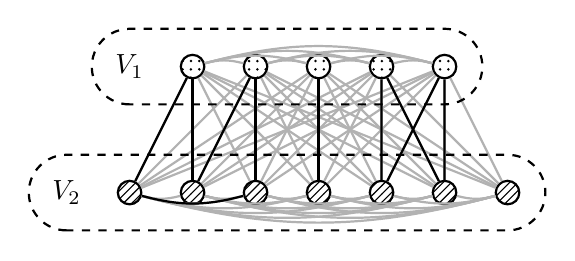
\begin{tikzpicture}[scale = 0.8,thick]
          \usetikzlibrary{patterns}
    		\tikzset{node/.style 2 args={draw, circle,draw=black,scale=0.9, label=#1:{\large #2}}};
    		\node[node={270}{},pattern=north east lines ] (0) at (0,0) {}; 
    		\node[node={270}{},pattern=north east lines ] (1) at (1,0) {}; 
    		\node[node={270}{},pattern = north east lines ] (2) at (2,0) {};
    		\node[node={270}{},pattern=north east lines ] (3) at (3,0) {};
    		\node[node={270}{},pattern=north east lines ] (4) at (4,0) {};
    		\node[node={270}{},pattern=north east lines ] (5) at (5,0) {};
    		\node[node={270}{},pattern=north east lines ] (6) at (6,0) {};
    		\node (a0) at (-1,0) {$V_2$};
    		\node[node={270}{},pattern=dots ] (7) at (1,2) {};
    		\node[node={270}{},pattern=dots ] (8) at (2,2) {};
    		\node[node={270}{},pattern=dots] (9) at (3,2) {};
    		\node[node={270}{} ,pattern=dots] (10) at (4,2) {};
    		\node[node={270}{},pattern=dots] (11) at (5,2) {};
    		\node (a7) at (0,2) {$V_1$};
    		
    		\foreach \j in {0,...,6}{
    			\foreach \i in {0,...,6}{
    				\ifthenelse{\i < \j}{}{
    					\draw (\i) edge[gray!60, bend left = 15] (\j);
    				}
    			}
    		}
    		
    		\foreach \j in {7,...,11}{
    			\foreach \i in {7,...,11}{
    				\ifthenelse{\i < \j}{}{
    					\draw (\i) edge[gray!60, bend right = 15] (\j);
    				}
    			}
    		}
    		\foreach \j in {0,...,6}{
    			\foreach \i in {7,...,11}{
    				\ifthenelse{\i < \j}{}{
    					\draw (\i) edge[gray!60] (\j);
    				}
    			}
    		}
    	
    		\draw (0)--(7);
    		\draw (7)--(1);
    		\draw (1)--(8);
    		\draw (8)--(2);
    		\draw (2) edge[bend left	 = 15] (0);
    		
    		\draw (3)--(9);
    		
    		\draw (4)--(10);
    		\draw (10)--(5);
    		\draw (5)--(11);
    		\draw (11)--(4);
    		
    	    \draw[dashed] \convexpath{a0,6}{0.6 cm};
    	    \draw[dashed] \convexpath{a7,11}{0.6 cm};
    		
    			
     	\end{tikzpicture}
    }
    \caption{Construction of $V_1$ and $V_2$ in Theorem~\ref{polydense}}
    \label{fig:polyDens}
 \end{figure}
 
 \begin{proof} We define a partition $\{V_1,V_2\}$ where $V_1$ (resp. $V_2$) contains vertices of color 1 (resp. 2). An example is given in Figure \ref{fig:polyDens}.
 Each vertex of degree $n-1$ has color 2. The graph $H$ of missing edges contains paths or cycles. The vertices on paths or cycles with an even number of vertices are colored alternating by 1 and 2. The vertices on paths or cycles with an odd number of vertices are colored alternating by 1 and 2 but starting with color 2. Thus cycles of odd size have two adjacent vertices of color 2.  The partition $\{V_1,V_2\}$ defined above is such that it contains $o$ missing edges in $V_2$ and $|V_2|$ is maximized among all such partitions.  
 Its density is equal to   $\frac{n-2}{2}- \frac{o}{n_2}$, where $n_2=|V_2|$. Denote by $d_{n-1}$ the number of vertices of~$G$ of degree $n-1$ and by $p_o$ the number of paths with an odd number of vertices (even length) among the missing edges. Thus $n_2=\frac12({n+d_{n-1}+p_o+o})$. We claim that there is no partition into two parts that has a higher density. 
 
 By Lemma~\ref{odd}, any partition into two sets contains at least $o$ missing edges inside the two parts. By construction we have maximized the number of vertices in the part with the missing edges among all partitions with the minimum number $o$ of missing edges, i.e., there is no partition into two parts  $\{V'_1,V'_2\}$ with $o$ missing edges all contained in $V'_2$ and $|V'_2|>|V_2|$. Hence, by Lemma~\ref{part1} and~\ref{part2}, it remains to show that any partition $\{V'_1,V'_2\}$ with $n'_2=|V_2|$ such that $n'_2=n_2+y$ with $o+x>o$ missing edges has a smaller density than  $\{V_1,V_2\}$.
 
 By definition of the partition $\{V_1,V_2\}$, it follows that $|E(H)|=2n_1-r+o$, where $r$ is the number of paths of odd length in $H$. For the partition $\{V'_1,V'_2\}$, it follows that $|E(H)|\leq 2(n_1-y)-r_1+(o+x)$, for some $r_1\geq r-x$ (number of vertices in $V'_1$ adjacent to only one edge in $H$). Observe that all non-edges have to either be among the $o+x$ missing edges in the partition or in the cut between $V'_1$ and $V'_2$. In the cut between $V'_1$ and $V'_2$, each vertex in $V'_1$ is adjacent to at most two such edges, and further every path of odd length either results in a vertex in $V'_1$ adjacent to only one edge  in $E(H)$ ($r_1$) or in a missing edge in $V'_2$, hence $r_1\geq r-x$. These inequalities imply that $y\leq x$, and hence the density of $\{V'_1,V'_2\}$ is at most $\frac{n-2}{2}- \frac{o+x}{n_2+y} \leq \frac{n-2}{2}- \frac{o+y}{n_2+y}\leq  \frac{n-2}{2}- \frac{o}{n_2}$.  Note that the last inequality follows from $o\leq {n_2}$, which simply holds since $H$ is of degree at most 2.
 %\todo[inline]{C added: In the following we justify that any partition $\{V'_1,V'_2\}$ with $n'_2=|V_2|$ such that $n'_2>n_2$ with 0 (respectively $o+y$) missing edges in $V'_1$ ($V'_2$)  has a smaller density than  $\{V_1,V_2\}$. More precisely, let consider that  $V'_2$ contains $x$ missing edges more than the partition  $\{V_1,V_2\}$ in  $V_2$ and $y$ more vertices. Since $H$ is of degree at most 2, we have $o\leq \frac{n_2}{2}$ and  $y\leq 2x$. Thus the density of  $\{V'_1,V'_2\}$ is equal to $\frac{n-2}{2}- \frac{o+x}{n_2+y} \leq \frac{n-2}{2}- \frac{o}{n_2}$.\\
%K: I expanded this to be more precise - I did not see how you got to  $y\leq 2x$ so quickly. Please check the above paragraph for correctness.}
%Overall, it follows that if $\frac{n-1}{2} - \frac{q}{n} \leq  \frac{n-2}{2}- \frac{o}{n_2}$, then an optimal solution of \MDGP{} on $G$  is $\{V_1,V_2\}$, otherwise it is the graph $G$. 
 \end{proof}


In the rest of the section  we consider graphs $G=(V,E)$ on $n$ vertices, $(n-4)$-regular, that is  $G=K_n-H$ where $H$ is a cubic graph. 
We show that \DGP~is NP-hard on $(n-4)$-regular graphs, by showing  a reduction from \UC{} on cubic graphs,  that is the complement of \textsc{Max Cut}.  This last problem on cubic graphs was proved  NP-hard and even not polynomial-time  1.003-approximable, unless P=NP \cite{BK99}.
 

\defprob{Min UnCut}{A graph $G=(V,E)$, an integer $k$.}{Does $G$ contain a partition of V into two parts $A, B$ such that the number of edges with both endpoints in the same part is at most $k$?}  

 

Since we did not find a reference for the following result in the literature. 

\begin{lemma}\label{perhapsknown}
\label{lem:borneUnCut}
Let $G=(V,E)$ be a cubic graph. There exists a partition $\{A,B\}$ of $G$ with a cut of size at least $|V|$ and it can be found in polynomial time.
\end{lemma}

\begin{proof}
Let $\mathcal{P} = \{A,B\}$ be a partition of $V$. Consider the following operation: if there is a vertex $v \in A$ (resp. $B$) with at least two neighbours in $A$ (resp. $B$) then $A = A \setminus \{v\} $ (resp. $B = B \setminus \{v\} $) and $B =  B \cup \{v\} $ (resp. $A = A \cup \{v\} $). Since the graph is cubic, this operation increases the number of edges between $A$ and $B$ by at least one. Since the number of edges is finite, we can repeat this operation until we obtain a partition $P'=\{A',B'\}$ with no vertex $v \in A'$ (resp. $B'$) with at least two neighbours in $A'$ (resp. $B'$). Since the graph is cubic, if every vertex in $A'$ (resp. $B'$) has at most one neighbour in $A'$, then it has at least two neighbours in $B'$ (resp. $A'$). Consequently $P'$ has a cut of size at least $ \frac{2(|A'| + |B'|)}{2} = |V|$.
\end{proof}

\begin{figure}
\begin{center}
    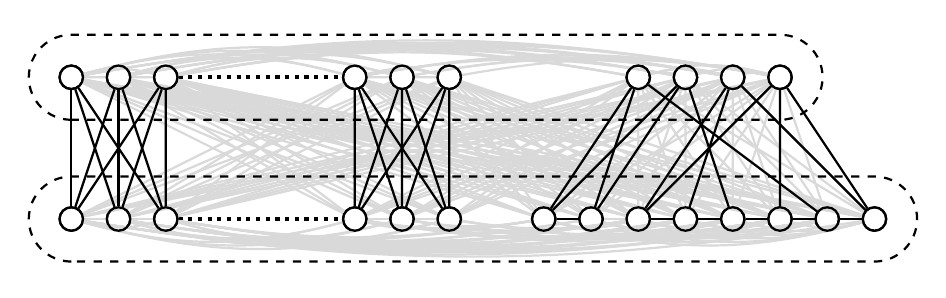
\begin{tikzpicture}[scale = 0.6,thick]
	\tikzset{node/.style 2 args={draw, circle,draw=black,scale=0.9, label=#1:{\large #2}}};
		\node[node={270}{} ] (0) at (0,0) {}; 
		\node[node={270}{} ] (1) at (1,0) {}; 
		\node[node={270}{} ] (2) at (2,0) {};
		
		
		\node[node={270}{} ] (3) at (6,0) {};
		\node[node={270}{} ] (4) at (7,0) {};
		\node[node={270}{} ] (5) at (8,0) {};
		
		
		
		
		\node[node={270}{} ] (7) at (0,3) {};
		\node[node={270}{} ] (8) at (1,3) {};
		\node[node={270}{} ] (9) at (2,3) {};
		
		
		\node[node={270}{} ] (10) at (6,3) {};
		\node[node={270}{} ] (11) at (7,3) {};
		\node[node={270}{} ] (12) at (8,3) {};
		
		\foreach \j in {0,...,5}{
			\foreach \i in {7,...,12}{
				\ifthenelse{\i < \j}{}{
					\draw (\i) edge[gray!30] (\j);
				}
			}
		}
		\draw (0) edge[gray!30, bend right = 15] (2);
		\draw (0) edge[gray!30, bend right = 15] (3);
		\draw (0) edge[gray!30, bend right = 15] (4);
		\draw (0) edge[gray!30, bend right = 15] (5);
		\draw (1) edge[gray!30] (2);
		\draw (1) edge[gray!30, bend right = 15] (3);
		\draw (1) edge[gray!30, bend right = 15] (4);
		\draw (1) edge[gray!30, bend right = 15] (5);
		
		\draw (2) edge[gray!30, bend right = 15] (4);
		\draw (2) edge[gray!30, bend right = 15] (5);
		
		\draw (3) edge[gray!30] (4);
		\draw (3) edge[gray!30, bend right = 15] (5);
		
		\draw (12) edge[gray!30, bend right = 15] (10);
		\draw (12) edge[gray!30, bend right = 15] (9);
		\draw (12) edge[gray!30, bend right = 15] (8);
		\draw (12) edge[gray!30, bend right = 15] (7);
		\draw (11) edge[gray!30] (10);
		\draw (11) edge[gray!30, bend right = 15] (9);
		\draw (11) edge[gray!30, bend right = 15] (8);
		\draw (11) edge[gray!30, bend right = 15] (7);
		
		\draw (10) edge[gray!30, bend right = 15] (8);
		\draw (10) edge[gray!30, bend right = 15] (7);
		
		\draw (9) edge[gray!30] (8);
		\draw (9) edge[gray!30, bend right = 15] (7);
		
		\draw (0) edge[gray!30] (1);
		\draw (12) edge[gray!30] (11);
		\draw (8) edge[gray!30] (7);
		\draw (4) edge[gray!30] (5);
		
		
		\draw[dotted, line width = 1.5] (2)--(3);
		\draw[dotted, line width = 1.5] (9)--(10);
		

	
		%-------------------------------------------------------
		

		
		\node[node={270}{} ] (a0) at (17,0) {}; 
		\node[node={270}{} ] (a2) at (13,0) {};
		\node[node={270}{} ] (a3) at (14,0) {};
		\node[node={270}{} ] (a4) at (10,0) {};
		\node[node={270}{} ] (a6) at (16,0) {};
		\node[node={270}{} ] (a7) at (15,0) {};
		\node[node={270}{} ] (a5) at (12,0) {};
		\node[node={270}{} ] (a1) at (11,0) {};
		
		\node[node={270}{} ] (a9) at (12,3) {};
		\node[node={270}{} ] (a10) at (13,3) {};
		\node[node={270}{} ] (a11) at (14,3) {};
		\node[node={270}{} ] (a12) at (15,3) {};
		
		\foreach \j in {0,...,7}{
			\foreach \i in {9,...,12}{
				\ifthenelse{\i < \j}{}{
					\draw (a\i) edge[gray!30] (a\j);
				}
			}
		}
		
		\foreach \i in {9,...,12}{
			\foreach \j in {9,...,12}{
				\ifthenelse{\i < \j}{}{
					\draw (a\i) edge[gray!30, bend right = 15] (a\j);
				}
			}
		}
		
		\draw (a4) edge[gray!30, bend right = 15] (a0);
		\draw (a4) edge[gray!30, bend right = 15] (a2);
		\draw (a4) edge[gray!30, bend right = 15] (a3);
		\draw (a4) edge[gray!30, bend right = 15] (a5);
		\draw (a4) edge[gray!30, bend right = 15] (a6);
		\draw (a4) edge[gray!30, bend right = 15] (a7);
		
		\draw (a1) edge[gray!30] (a5);
		\draw (a1) edge[gray!30, bend right = 15] (a0);
		\draw (a1) edge[gray!30, bend right = 15] (a2);
		\draw (a1) edge[gray!30, bend right = 15] (a3);
		\draw (a1) edge[gray!30, bend right = 15] (a6);
		\draw (a1) edge[gray!30, bend right = 15] (a7);
		
		\draw (a5) edge[gray!30, bend right = 15] (a0);
		\draw (a5) edge[gray!30, bend right = 15] (a3);
		\draw (a5) edge[gray!30, bend right = 15] (a6);
		\draw (a5) edge[gray!30, bend right = 15] (a7);
		
		\draw (a2) edge[gray!30, bend right = 15] (a0);
		\draw (a2) edge[gray!30, bend right = 15] (a6);
		\draw (a2) edge[gray!30, bend right = 15] (a7);
		
		\draw (a3) edge[gray!30, bend right = 15] (a0);
		\draw (a3) edge[gray!30, bend right = 15] (a6);
		
		\draw (a7) edge[gray!30, bend right = 15] (a0);
		
		
		
		
		\foreach \i in {9,...,12}{
			\foreach \j in {7,...,12}{
				\ifthenelse{\i < \j}{}{
					\draw (a\i) edge[gray!30, bend right = 10] (\j);
				}
			}
		}
	
		\foreach \i in {0,...,7}{
			\foreach \j in {0,...,5}{
				\ifthenelse{\i < \j}{}{
					\draw (a\i) edge[gray!30, bend left = 9] (\j);
				}
			}
		}
	
		\foreach \i in {9,...,12}{
			\foreach \j in {0,...,5}{
					\draw (a\i) edge[gray!30] (\j);
			}
		}
	
		\foreach \i in {0,...,7}{
			\foreach \j in {7,...,12}{
				\draw (a\i) edge[gray!30] (\j);
			}
		}

		\draw[line width=0.8pt] (a0)--(a12);
		\draw[line width=0.8pt]  (a2)--(a3);
		\draw[line width=0.8pt]  (a4)--(a9);
		\draw[line width=0.8pt]  (a6)--(a7);
		\draw[line width=0.8pt]  (a5)--(a11);
		\draw[line width=0.8pt]  (a10)--(a1);
		\draw[line width=0.8pt]  (a0)--(a6);
		\draw[line width=0.8pt]  (a3)--(a7);
		\draw[line width=0.8pt]  (a12)--(a7);
		\draw[line width=0.8pt]  (a12)--(a5);
		\draw[line width=0.8pt]  (a2)--(a5);
		\draw[line width=0.8pt]  (a2)--(a11);
		\draw[line width=0.8pt]  (a0)--(a11);
		\draw[line width=0.8pt]  (a3)--(a10);
		\draw[line width=0.8pt]  (a4)--(a10);
		\draw[line width=0.8pt]  (a4)--(a1);
		\draw[line width=0.8pt]  (a9)--(a1);
		\draw[line width=0.8pt]  (a9)--(a6);
		
		\foreach \j in {0,...,2}{
			\foreach \i in {7,...,9}{
				\ifthenelse{\i < \j}{}{
					\draw (\i) edge (\j);
				}
			}
		}
		
		\foreach \j in {3,...,5}{
			\foreach \i in {10,...,12}{
				\ifthenelse{\i < \j}{}{
					\draw (\i) edge (\j);
				}
			}
		}
		
		\draw[dashed] \convexpath{0,a0}{0.9 cm};
		\draw[dashed] \convexpath{7,a12}{0.9 cm};
		
		
		\node[node={270}{} ] (0) at (0,0) {}; 
		\node[node={270}{} ] (1) at (1,0) {}; 
		\node[node={270}{} ] (2) at (2,0) {};
		
		
		\node[node={270}{} ] (3) at (6,0) {};
		\node[node={270}{} ] (4) at (7,0) {};
		\node[node={270}{} ] (5) at (8,0) {};
		
		
		
		
		\node[node={270}{} ] (7) at (0,3) {};
		\node[node={270}{} ] (8) at (1,3) {};
		\node[node={270}{} ] (9) at (2,3) {};
		
		
		\node[node={270}{} ] (10) at (6,3) {};
		\node[node={270}{} ] (11) at (7,3) {};
		\node[node={270}{} ] (12) at (8,3) {};
		
		\node[node={270}{} ] (a0) at (17,0) {}; 
		\node[node={270}{} ] (a2) at (13,0) {};
		\node[node={270}{} ] (a3) at (14,0) {};
		\node[node={270}{} ] (a4) at (10,0) {};
		\node[node={270}{} ] (a6) at (16,0) {};
		\node[node={270}{} ] (a7) at (15,0) {};
		\node[node={270}{} ] (a5) at (12,0) {};
		\node[node={270}{} ] (a1) at (11,0) {};
		
		\node[node={270}{} ] (a9) at (12,3) {};
		\node[node={270}{} ] (a10) at (13,3) {};
		\node[node={270}{} ] (a11) at (14,3) {};
		\node[node={270}{} ] (a12) at (15,3) {};
	\end{tikzpicture}
    \caption{The construction of $G'$ in Definition~\ref{denseNPdef}}
    \label{fig:hardDens}
    \end{center}
\end{figure}

\begin{definition}\label{denseNPdef}
Let $I = (G,k)$ be an instance of \UC~ where $G=(V,E)$ is a cubic graph. We define the construction $\sigma$ transforming the graph $G$ into the graph $G':= (V',E') =\sigma(G)$ (see Figure \ref{fig:hardDens}) as follows:
\begin{itemize}
    \item let $G_0=(V_0,E_0)$ be the union of  $\frac{n^2 - n}{6}$ copies of $K_{3,3}$ (see remark below). Thus $G_0$ is a cubic bipartite graph with $n^2 - n$ vertices and $V_0$ is the union of two independent sets $L, R$ such that $|L|=|R|$.
    \item let $G_1 = (V \cup V_0, E \cup E_0)$.
    \item let $G' = \overline{G_1}$.
\end{itemize}
 
\end{definition}

\begin{remark}
Note that  we can assume that the number of vertices of a cubic graph $G$  is a multiple of $6$. Since $G$ is cubic, $n$ is a multiple of 2.
If $n$ is not a multiple of 3, we consider the instance $I_{triple}$ defined as follows: $G_{triple}$ is the union of 3 copies of $G$ and $k_{triple}=3k$, and thus in the new instance $I_{triple}$ the graph has $3n$ vertices. 
\end{remark}

Let $n=|V|$, $m=|E|$,  $n'=|V'|$ and $m'=|E'|$. Remark that $n' = n^2$, and  $G'$ is a $(n'-4)$-regular graph. 

Since we reduce from {Min UnCut} on cubic graphs, we use the following straight forward observation on any partition in such graphs.
\begin{lemma} For any cubic graph $G$ and any $\{A,B\}$   partition of $V$, we have 
$ |A| + \frac{2}{3}\cdot |E(B)| = |B| + \frac{2}{3} \cdot |E(A)|$, 
where $E(A)$, resp.~$E(B)$, are the set of edges with both endpoints in $A$, resp~$B$.
\label{lem:interneexterne}
\end{lemma}

\begin{proof}
Since the graph $G$ is cubic, 
$E(A,B)  = 3\cdot |A| - 2 \cdot|E_A|  = 3\cdot |B| - 2 \cdot |E_B|$.
We can deduce that $|A| + \frac{2}{3} \cdot |E_B| = |B| + \frac{2}{3} \cdot |E_A|$ 
\end{proof}


\begin{theorem}\label{denseNP}
\DGP{} is NP-complete on $(n-4)$-regular graphs with $n$ vertices.
\end{theorem}

\begin{proof}
Let $I=(G=(V,E),k)$ be an instance of \UC,  where $G$ is a cubic graph.  Consider the following instance $I'$ of \DGP{} on the graph $G' = \sigma(G)$ and $d=\frac{n^2}{2} - 1 - \frac{2k}{n^2}$. We claim that $I= (G,k)$ is a yes-instance of \UC~ if and only if $I' = (G',d)$ is a yes-instance of \DGP.
\medskip

Let $\{A,B\}$ be a partition of $V$ whose  uncut value is at most $k$. Since $V_0=L\cup R$, where $L,R$ are independent sets in $G_0$ such that $|L|=|R|$, the sets $L,R$ form two cliques of the same size in $G'$. Let $A' = A \cup L$ and $B' = B \cup R$  and $\mathcal{P}=\{A',B'\}$ be a partition of $G'$. 

Let ${M}_{A'}$ and ${M}_{B'}$, be the set of missing edges in $G'[A']$ and $G'[B']$, respectively. 
Due to the construction of $G'$, there is no missing edge  between $A$ and $L$ and between $B$ and $R$. Thus all missing edges are inside $G'[A\cup B]$, then $|{M}_{A'}| + |{M}_{B'}| = k$. Thus, the density of the partition $\mathcal{P}$ is: 
$$ d(\mathcal{P}) = \frac{|A'|-1}{2} - \frac{|{M}_{A'}|}{|A'|} + \frac{|B'|-1}{2} - \frac{|{M}_{B'}|}{|B'|} 
       = \frac{n^2-2}{2} - \frac{|{M}_{A'}|}{|A'|} - \frac{|{M}_{B'}|}{|B'|}
$$
We will prove in the following that  $d(\mathcal{P})
\geq d=\frac{n^2}{2} - 1 - \frac{2k}{n^2}$ that is equivalent to proving that $\frac{|{M}_{A'}|}{|A'|} + \frac{|{M}_{B'}|}{|B'|} \leq \frac{2(|M_{A'}|+|M_{B'}|)}{|A'|+|B'|}$.


Thus the difference 
$$  \frac{2(|M_{A'}|+|M_{B'}|)}{|A'|+|B'|} - \left(\frac{|M_{A'}|}{|A'|} + \frac{|M_{B'}|}{|B'|}\right)=$$
$$=\frac{1}{|A'|+|B'|} \left( 2|M_{A'}|+2|M_{B'}| - \frac{|A'|+|B'|}{|A'|} |M_{A'}|-\frac{|A'|+|B'|}{|B'|} |M_{B'}|\right)=$$
$$=\frac{1}{|A'|+|B'|} \frac{1}{|A'|} \frac{1}{|B'|} (|A'||B'| |M_{A'}|+ |A'||B'| |M_{B'}|-|B'|^2 |M_{A'}|- |A'|^2 |M_{B'}|)=
$$
$$ =\frac{1}{|A'|+|B'|} \frac{1}{|A'|} \frac{1}{|B'|} (|A'|-|B'|)(|B'||M_{A'}|-|A'||M_{B'}|)
$$

Wlog we can consider that $|A'|\geq |B'|$, that implies $|B'|\leq \frac{n^2}{2}$.
From Lemma~\ref{lem:interneexterne}  for the cubic graph $G_1$ and partition $\{A', B'\}$,  we have 
$|A'|+ \frac{2}{3}\cdot |M_{B'}| = |B'| + \frac{2}{3} \cdot |M_{A'}|$. Using that $|A'|=n^2-|B'|$ and $|M_{A'}|=k-|M_{B'}|$, we have $n^2-|B'|+ \frac{2}{3}\cdot |M_{B'}| = |B'| + \frac{2}{3} \cdot (k-|M_{B'}|)$  and thus $ |M_{B'}|= \frac{3}{4} (2 |B'|+ \frac{2}{3} k-n^2)$.

Thus, 
$$|B'||M_{A'}|-|A'||M_{B'}|= |B'| (k-|M_{B'}|) - (n^2-|B'|)|M_{B'}|=|B'|k-n^2 |M_{B'}|=$$
$$=|B'|k-n^2\frac{3}{4} \left(2 |B'|+ \frac{2}{3} k-n^2\right)=\left(|B'|-\frac{n^2}{2}\right)\left(k-\frac{3n^2}{2}\right)$$
Since $|B'|\leq \frac{n^2}{2}$ and $k \leq  \frac{n}{2}\leq \frac{3n^2}{2}$ we can conclude  that 
$$  \frac{2(|M_{A'}|+|M_{B'}|)}{|A'|+|B'|} - \left(\frac{|M_{A'}|}{|A'|} + \frac{|M_{B'}|}{|B'|}\right) \geq 0$$

Thus, the partition $\mathcal{P}=\{A',B'\}$  has the density $d(\mathcal{P})
\geq d=\frac{n^2}{2} - 1 - \frac{2k}{n^2}$.
 


 \bigskip
 Let $\mathcal{P'}$ be a partition of $G'$ of density $d(\mathcal{P'}) \geq d = \frac{n^2-2}{2} - \frac{2k}{n^2}$. We will prove that $\mathcal{P'}$ has exactly two parts $A'$ and $B'$ such that $A = A' \cap V$ and $B = B' \cap V$ is a partition of $G$ whose uncut value is at most $k$.

Suppose that $|\mathcal{P'}| \geq 3$. Then, using Lemma~\ref{lem:densMax}, we have $d(\mathcal{P'}) \leq \frac{n^2 - |\mathcal{P'}|}{2} \leq \frac{n^2-3}{2} = \frac{n^2-2}{2} - \frac{1}{2}$. Since $k \leq \frac{n}{2}$ and $n \geq 6$ then $\frac{2k}{n^2} < \frac{1}{2}$. Then $d(\mathcal{P'}) < \frac{n^{2}-2}{2} - \frac{2k}{n^2} = d$ which is a contradiction. Then $|\mathcal{P'}| < 3$.

Suppose that $|\mathcal{P'}| = 1$. Since $G'$ is $(n^2-4)$-regular, its density is $d(\mathcal{P'}) = \frac{n^2-1}{2} - \frac{3}{2} = \frac{n^2-2}{2} - 1 < \frac{n^2-2}{2} - \frac{2k}{n^2} = d$ which is a contradiction. Then $|\mathcal{P'}| > 1$. We conclude that $|\mathcal{P}| = 2$.

Let $A'$ and $B'$ be the two parts of $\mathcal{P}$. Let ${M}_{A'}$, resp. ${M}_{B'}$, be the set of missing edges in $G'[A']$, resp. $G'[B']$. Remark that if $|M_{A'}| + |M_{B'}| \leq k$ then $|M_{A}| + |M_{B}| \leq k$ and then there is a cut of size at least $k$ between $A$ and $B$ in $G$. What it remains to prove is that $|M_{A'}| + |M_{B'}| \leq k$.



As a first step we will show the following inequality we need later $\frac{|{M}_{A'}| + |{M}_{B'}|}{\frac{n^2}{2} + \frac{|{M}_{A'}| + |{M}_{B'}|}{3}} \leq \frac{|{M}_{A'}|}{|A'|} + \frac{|{M}_{B'}|}{|B'|}$. In order to prove this, we consider the following difference 
$$
    \frac{|{M}_{A'}|}{|A'|} + \frac{|{M}_{B'}|}{|B'|} - \frac{|{M}_{A'}|+|{M}_{B'}|}{\frac{|A'|+|B'|}{2} + \frac{|{M}_{A'}| + |{M}_{B'}|}{3}} 
$$

By removing the denominator we get 
$$
    |{M}_{A'}||B'|\left(\frac{|A'| + |B'|}{2} + \frac{|{M}_{A'}|+|{M}_{B'}|}{3}\right) + |{M}_{B'}||A'|\left(\frac{|A'| + |B'|}{2} + \frac{|{M}_{A'}|+|{M}_{B'}|}{3}\right) 
$$    
$$    
    - (|{M}_{A'}| + |{M}_{B'}|)|A'||B'| =
$$     
$$     
     = |{M}_{A'}||B'| \left(\frac{|B'|}{2} + \frac{|{M}_{A'}|}{3} + \frac{|{M}_{B'}|}{3} - \frac{|A'|}{2}\right) + |{M}_{B'}||A'|\left(\frac{|A'|}{2} + \frac{|{M}_{B'}|}{3} + \frac{|{M}_{A'}|}{3} - \frac{|B'|}{2}\right) =
$$

From Lemma~\ref{lem:interneexterne}  for the cubic graph $G_1$ and partition $\{A', B'\}$,  we have $|A'| + \frac{2}{3}|{M}_{B'}| = |B'| + \frac{2}{3}|{M}_{A'}|$, which implies that $\frac{|A'|}{2} = \frac{|B'|}{2} + \frac{|{M}_{A'}|}{3} - \frac{|{M}_{B'}|}{3}$ and $\frac{|B'|}{2} = \frac{|A'|}{2} + \frac{|{M}_{B'}|}{3} - \frac{|{M}_{A'}|}{3}$ and then we get 
$$
    = |{M}_{A'}||B'| \left(\frac{|B'|}{2} + \frac{|{M}_{A'}|}{3} + \frac{|{M}_{B'}|}{3} - \left(\frac{|B'|}{2} + \frac{|{M}_{A'}|}{3} - \frac{|{M}_{B'}|}{3}\right)\right)
$$    
$$    
     + |{M}_{B'}||A'|\left(\frac{|A'|}{2} + \frac{|{M}_{B'}|}{3} + \frac{|{M}_{A'}|}{3} - \left(\frac{|A'|}{2} + \frac{|{M}_{B'}|}{3} - \frac{|{M}_{A'}|}{3}\right)\right) =
$$
$$
    = |{M}_{A'}||B'|\frac{2|{M}_{B'}|}{3} + |{M}_{B'}||A'|\frac{2|{M}_{A'}|}{3}
$$
Since $|{M}_{A'}|$, $|{M}_{B'}|$, $|A'|$ and $|B'|$ are positive integers then  $\frac{|{M}_{A'}|}{|A'|} + \frac{|{M}_{B'}|}{|B'|} - \frac{|{M}_{A'}| + |{M}_{B'}|}{\frac{n^2}{2} + \frac{|{M}_{A'}| + |{M}_{B'}|}{3}} \geq 0$. We conclude that $\frac{|{M}_{A'}| + |{M}_{B'}|}{\frac{n^2}{2} + \frac{|{M}_{A'}| + |{M}_{B'}|}{3}} \leq \frac{|{M}_{A'}|}{|A'|} + \frac{|{M}_{B'}|}{|B'|}$.

\medskip


Finally, we  show that $|{M}_{A'}| + |{M}_{B'}| \leq k$ using the previous inequality. Let $x= |{M}_{A'}| + |{M}_{B'}|$. In order to finalize  the proof, we suppose that $x> k$ and we will arrive at a contradiction, that is   $d(\mathcal{P'}) < d$. Consider the following difference
$$
d - d(\mathcal{P'}) = \frac{n^2 - 2}{2} - \frac{2k}{n^2} - \left(\frac{n^2 - 2}{2} - \frac{|{M}_{A'}|}{|A'|} - \frac{|{M}_{B'}|}{|B'|}\right) = \frac{|{M}_{A'}|}{|A'|} + \frac{|{M}_{B'}|}{|B'|} - \frac{2k}{n^2}
$$
Since $\frac{x}{\frac{n^2}{2} + \frac{x}{3}} \leq \frac{|{M}_{A'}|}{|A'|} + \frac{|{M}_{B'}|}{|B'|}$ then
$$
d - d(\mathcal{P'}) \geq \frac{x}{\frac{n^2}{2}+\frac{x}{3}} - \frac{2k}{n^2} = \frac{x\cdot n^2 - k \cdot n^2 -\frac{2x\cdot k}{3}}{(\frac{n^2}{2}+\frac{x}{3}) \cdot n^2}
$$
Since $x$ and $k$ are integers, then $x\geq k+1$, and by removing the denominator, we get 
$$
    \geq (k+1) \cdot (n^2 - \frac{2}{3}\cdot k) - k\cdot n^2 = n^2 - \frac{2}{3}\cdot k^2 - \frac{2}{3}\cdot k
$$ 

Since $k \leq \frac{n}{2}$ it follows that $n^2 - \frac{2}{3}\cdot k^2 - \frac{2}{3}\cdot k > 0$. This finally gives $d(\mathcal{P'}) < d$, a contradiction to the choice of $\mathcal P'$ as partition with density at least $d$, and we hence conclude that $|{M}_{A'}| + |{M}_{B'}| \leq k$.

Overall, it follows that if $d(\mathcal{P'}) \geq \frac{n^{'}-2}{2} - \frac{2k}{n^2}$ then there is a partition $\{A,B\}$ with an uncut of size at most $k$.
\end{proof}

At the end of this section we show that a partition into three cliques provides a good approximation of the problem.

\begin{lemma}
\label{lem:borneDensNReg} Let $G=(V,E)$ be a $(n-4)$-regular graph and   $\mathcal{P}$ any partition of $V$. Then $d(\mathcal{P}) \leq \frac{n}{2} - 1$.
\end{lemma}
\begin{proof}
If $|\mathcal{P}| = 1$ then $d(\mathcal{P}) = \frac{n-4}{2}$. Suppose that $|\mathcal{P}| \geq 2$, the density is maximized when for every $P \in \mathcal{P}$, $G[P]$ is a clique. Then $d(\mathcal{P}) = \sum\limits_{P \in \mathcal{P}}$ $\frac{|P| - 1}{2} \leq \frac{n}{2} - 1$.
\end{proof}

\begin{theorem}
There is an efficient  polynomial time approximation scheme for \MDGP{} on $(n-4)$-regular graphs.
\end{theorem}
\begin{proof}
Let $I=G$  be a graph on $n$ vertices and $(n-4)$-regular, instance of \MDGP. Let $\overline{G}$ be the complementary graph of $G$. By Brooks' theorem, we know that there is a 3-coloration of $\overline{G}$ that can be found in polynomial time \cite{Karloff89}.  

We establish in the following an eptas. Given $\varepsilon>0$, consider two cases. If $n\geq 3+\frac{1}{\varepsilon}$, then
let $\mathcal{P}$ be a partition, that corresponds to a 3-coloration of $\overline{G}$,  that is each part is a clique in  $G$. Then $d(\mathcal{P}) = \frac{n}{2} - \frac{3}{2}$. By Lemma~\ref{lem:borneDensNReg} we know that $opt(I) \leq \frac{n}{2} - 1$. Thus $d(\mathcal{P}) \geq \frac{n/2-1}{1+\varepsilon}\geq \frac{opt(I)}{1+\varepsilon}$. 

Otherwise, that is 
$n < 3+\frac{1}{\varepsilon}$, enumerate all the partitions of $G$ and consider the best one. Since the number of partitions of $G$ is the Bell number of order $|V|=n$, $B_n$, and that $B_n\leq n^n$, we get an optimal solution in time $O((1/\varepsilon)^ {1/\varepsilon})$. \end{proof}

 
\section{Conclusion}
  In order to have a better understanding of the complexity of  \MDGP{} it would be nice to study it on other graph classes.  It was proved to be polynomial-time solvable on trees, but the complexity on graphs of bounded treewidth  remains open. Moreover no result exists on split graphs. 
  Concerning the approximation, no lower bound was established, it would be nice to improve the 2-approximation algorithm or to show that no polynomial-time approximation scheme exist on general instances. 

\bibstyle{plainurl} 
\bibliography{references.bib}

\end{document}